\documentclass[aspectratio=169]{beamer}

\usetheme{default}
\usecolortheme{default}

\usepackage{amsmath,amssymb}
\usepackage{mathtools}
\usepackage{comment}
\usepackage{tikz}
\usetikzlibrary{fit,calc,positioning,arrows.meta,backgrounds,shadows.blur,shapes.geometric,decorations.pathreplacing}
\usepackage{svg}
\usepackage{listings}
\lstdefinestyle{p4style}{
  language=C,
  basicstyle=\ttfamily\fontsize{6}{4.8}\selectfont,
  keywordstyle=\bfseries,
  showstringspaces=false,
  breaklines=false,
  frame=none,
  xleftmargin=0pt,
  aboveskip=1pt,
  belowskip=1pt,
  columns=fixed,
  morekeywords={header,parser,control,table,action,state,transition,
    select,apply,extract,bit,typedef,struct,inout,out,packet_in,
    default_action,key,actions,size,lpm,mark_to_drop,isValid,NoAction,const},
}
\lstdefinestyle{haskellstyle}{
  language=Haskell,
  basicstyle=\ttfamily\fontsize{5.8}{7.0}\selectfont,
  keywordstyle=\bfseries,
  showstringspaces=false,
  breaklines=false,
  frame=none,
  xleftmargin=0pt,
  aboveskip=1pt,
  belowskip=1pt,
  columns=fullflexible,
  keepspaces=true,
}
\usepackage[style=numeric,backend=biber]{biblatex}
\addbibresource{references.bib}

\newbibmacro*{authorurlcite:body}{%
  \printnames{author}%
  \setunit{\addperiod\space}%
  \iffieldundef{url}
    {\printfield[citetitle]{title}}
    {\href{\thefield{url}}{\printfield[citetitle]{title}}}%
  \iffieldundef{year}
    {}
    {\setunit{\addperiod\space}\printfield{year}}%
  \iffieldundef{doi}
    {\iffieldundef{url}
       {}
       {\setunit{\addperiod\space}URL:\space\href{\thefield{url}}{\nolinkurl{\thefield{url}}}}}
    {\setunit{\addperiod\space}DOI:\space\href{https://doi.org/\thefield{doi}}{\nolinkurl{\thefield{doi}}}}%
}

\DeclareCiteCommand{\footauthorurlcite}[\mkbibfootnote]
  {\usebibmacro{prenote}}
  {\usebibmacro{authorurlcite:body}}
  {\multicitedelim}
  {\usebibmacro{postnote}}

\newif\ifextendedslides
\ifnum\pdfstrcmp{\jobname}{Extended}=0
  \extendedslidestrue
\else
  \extendedslidesfalse
\fi

\ifextendedslides
  \includecomment{hidden}
\else
  \excludecomment{hidden}
\fi

\newcommand{\grisetteframecite}{%
  \footnote[frame]{%
    Sirui Lu and Rastislav Bod\'{\i}k. \emph{Grisette: Symbolic Compilation as a Functional Programming Library}. 2023.
    DOI:\space\href{https://doi.org/10.1145/3571209}{10.1145/3571209}.%
  }%
}

\setbeamertemplate{navigation symbols}{}
\setbeamertemplate{footline}{}

\usepackage[T1]{fontenc}
\usepackage{zi4} % Inconsolata monospace font
\usepackage{helvet} % Helvetica for sans-serif

% Styles shared with arch.tex
\definecolor{uiLight}{HTML}{F6F8FA}
\definecolor{uiBorder}{HTML}{B8C2CC}
\definecolor{uiText}{HTML}{2F363D}
\definecolor{cexFill}{HTML}{FFF4F4}
\definecolor{cexBorder}{HTML}{E57373}
\definecolor{highColor}{HTML}{1976D2}
\definecolor{highFill}{HTML}{E3F2FD}

\tikzset{
block/.style={
draw=uiBorder,
fill=uiLight,
rounded corners=2mm,
line width=0.9pt,
blur shadow={shadow blur steps=4,shadow opacity=12},
align=center,
minimum width=6.2cm,
minimum height=1.35cm,
font=\sffamily\bfseries,
text=uiText
},
instblock/.style={
draw=uiBorder,
fill=uiLight,
rounded corners=2mm,
line width=0.9pt,
blur shadow={shadow blur steps=4,shadow opacity=12},
align=center,
minimum width=2.6cm,
minimum height=0.8cm,
font=\sffamily\bfseries,
text=uiText
},
cexblock/.style={
draw=cexBorder,
fill=cexFill,
rounded corners=2mm,
line width=1.1pt,
blur shadow={shadow blur steps=4,shadow opacity=12},
align=center,
minimum width=4.7cm,
minimum height=1.05cm,
font=\sffamily\bfseries,
text=uiText
},
flow/.style={
-{Latex[length=3.0mm]},
draw=uiText,
line width=1.0pt
},
highlighted block/.style={
block,
draw=highColor,
fill=highFill,
line width=1.8pt,
text=highColor
},
highlighted flow/.style={
flow,
draw=highColor,
line width=1.8pt
},
dimmed/.style={
opacity=0.25,
text opacity=0.25
},
legendBox/.style={
draw=uiBorder,
fill=white,
rounded corners=1mm,
font=\sffamily\bfseries\small,
inner sep=6pt,
align=left,
blur shadow={shadow blur steps=2,shadow opacity=10},
text width=4cm
}
}


\title{P4Check: a P4 Verification Tool}
% \subtitle{MNS Status Update}
\author{Tommaso Pacciani}
\date{\today}

\newcommand{\architecturelegenditem}[2]{%
  \ifnum#1<#2\relax
    \phantom{\ifcase#2\or 1. Concrete Execution\or 2. Verification\or 3. Symbolic Execution\fi}%
  \else
    \ifcase#2\or 1. Concrete Execution\or 2. Verification\or 3. Symbolic Execution\fi
  \fi
}

\newcommand{\architecturelegend}[1]{%
  \architecturelegenditem{#1}{1}\\
  \architecturelegenditem{#1}{2}\\
  \architecturelegenditem{#1}{3}%
}

\begin{document}

\begin{frame}
  \titlepage
  \begin{tikzpicture}[remember picture,overlay]
    \node[anchor=south, xshift=-2.5cm, yshift=1cm] at (current page.south) {
      \includesvg[height=1.35cm]{uva_logo.svg}
    };
    \node[anchor=south, xshift=2.5cm, yshift=0.425cm] at (current page.south) {
      \includesvg[height=2.5cm]{fns_logo.svg}
    };
  \end{tikzpicture}
\end{frame}

\setbeamertemplate{footline}{%
  \begin{beamercolorbox}[wd=\paperwidth,ht=3ex,dp=1.5ex,leftskip=2ex,rightskip=2ex]{page number in head/foot}%
    \raisebox{-0.1cm}{\includegraphics[height=0.45cm]{uvalogo_tag_p.eps}}%
    \hspace{0.05cm}%
    \includegraphics[height=0.35cm]{smallLogo.pdf}%
    \hfill%
    \insertframenumber{} / \inserttotalframenumber%
  \end{beamercolorbox}%
}

\begin{frame}{What is P4? \footauthorurlcite{10.1145/2656877.2656890}}
    \begin{columns}[T]
        
        % Left Column: What is P4
        \begin{column}{0.48\textwidth}
            \begin{itemize}\setlength\itemsep{8pt}
                \item A \textbf{domain-specific language} for programming the \textbf{data plane} of network devices (switches, SmartNICs, \dots).
                \item \textbf{Protocol independent} \& \textbf{programmable} \textbf{line rate} packet transformations (e.g., 12.8+ Tbps).
                \item Library (V1Model, PSA, TNA) + (linux XDP,  ) + Possibly other vendor specific 
             \end{itemize}
        \end{column}
        
        % Right Column: The Problem
        \begin{column}{0.48\textwidth}
        \only{

          \begin{alertblock}{The Problem}
                P4 programs are \textbf{difficult to test}. Programs are \textbf{device-specific} and behavior depends on runtime-installed \textbf{table entries}.
            \end{alertblock}
            
            \vspace{0.5em}
            \begin{itemize}\setlength\itemsep{6pt}
                \item \textbf{Lack of modularity} 

              \item Requires dedicating specific hardware targets to run tests.
            \end{itemize}}<2>
        \end{column}
        
    \end{columns}
\end{frame}


% \begin{frame}
% \frametitle{What is P4 \footauthorurlcite{10.1145/2656877.2656890}}
% \begin{itemize}\setlength\itemsep{3pt}
% \item A \textbf{domain-specific language} for programming the
%       \textbf{data plane} of network devices (switches, smartNICs, \dots)
% \item packets \textbf{transformed} at line rate [TODO add nums with ref]
% \item Target-independent specification compiled to
%       device-specific back-ends (V1Model, PSA, TNA, \ldots)
% \end{itemize}
% \cite{p4}


%   \cite{p4}

%   \begin{block}{The Problem}
%     P4 programs are \textbf{difficult to test} because behavior is \textbf{device-specific} and depends heavily on the control plane \textbf{table entries} installed at runtime.
    
%     \vspace{0.5em}
%     \textbf{Key Testing Challenges:}
%     \begin{itemize}
%         \item Requires devoting specific hardware targets to run tests.
%         \item P4 programs act as \textbf{monolithic blocks}. 
%         \item Lack of modularity
%     \end{itemize}
%   \end{block}
% \end{frame}



\begin{frame}{State of the Art in P4 Verification}
  \vspace{-0.5em}
  
  \begin{block}{Stateless / Single-Packet Verification}
    \small
    \textbf{Tools:} p4v \cite{10.1145/3230543.3230582}, Vera, ASSERT-P4 \cite{10.1145/3185467.3185499} \\
    \textcolor{red!70!black}{\textbf{Limitations:}} stateless, closed source, soundness and completeness.
  \end{block}
  
  \begin{block}{Stateful / Temporal Verification}
    \small
    \textbf{Tools:} p4tv \cite{10.5555/3767955.3767968} \\
    \textcolor{red!70!black}{\textbf{Limitation:}} Supports LTL/CTL across packets, but lacks support for relating internal program components
  \end{block}
  
  \begin{block}{Formal Semantics \& Test Generation}
    \small
    \textbf{Tools:} p4testgen \cite{10.1145/3603269.3604834}, P4 in Rocq \cite{10.4230/LIPIcs.ITP.2023.32}, HOL4P4 \\
    \textcolor{red!70!black}{\textbf{Limitation:}} Header stacks \& Tofino, lack of tooling for verification with dedicated, user-friendly spec languages on top of these semantics.
  \end{block}
\end{frame}


\begin{frame}{P4Check}                                           
                                                                                
  \begin{columns}[T]                                                            
                                                                                
  \begin{column}{0.55\textwidth}                                                
                                                                                
  % \begin{block}{What is P4Check?}                                                        
  A \textbf{symbolic execution engine} for P4                                          
  \begin{itemize}\setlength\itemsep{2pt}                                        
    \item Written in Haskell (${\sim}10$k LOC), built on \textbf{Grisette}\grisetteframecite
  (a symbolic evaluation library)                                              
    \item \textbf{Mode-polymorphic interpreter:} one codebase, two modes ---    
  concrete and symbolic                          
    \item Targets V1Model, PSA, and TNA architectures                          
  \end{itemize}                                                                 
  % \end{block}                                                              
                                                                                
  \end{column}                                                                  
  
  \begin{column}{0.42\textwidth}                                                
                                                                           
  \begin{block}{Capabilities}
  \small
  \begin{enumerate}\setlength\itemsep{3pt}
    \item[\checkmark] \textbf{Invalid-access detection} --- finds reads of      
  invalid headers via symbolic exploration                                      
    \item[\checkmark] \textbf{Property verification} --- checks user-specified
  assertions (safety, reachability, field invariants)                           
    \item[\checkmark] \textbf{Multi-packet reasoning} --- CTL model checking
  over stateful register/counter interactions
  
  \item[\checkmark] \textbf{Steppable debugger}
  \end{enumerate}                                                          
  \end{block}                                                                   
                                                                           
  \end{column}
  \end{columns}
                                                                                
\end{frame}


              

\section{Background}
\begin{frame}
\centering
\LARGE Background
\end{frame}

\begin{frame}[fragile]
  \frametitle{Symbolic Execution}
  \footauthorurlcite{10.1145/360248.360252}

  \small
  \begin{columns}[T]
    \begin{column}{0.22\textwidth}
      \footnotesize
      \textbf{Program:}
      \smallskip

      \begin{tabular}{@{}r@{\;}l@{}}
      1: & $\mathit{extract}(\mathit{ipv4})$ \\
      2: & $\mathit{if}\;(\mathit{ipv4.ttl} > 1)$ \\
      3: & \quad $\mathit{ipv4.ttl} :=$ \\
         & \quad\quad $\mathit{ipv4.ttl} - 1$ \\
      4: & $\mathit{else}$ \\
      5: & \quad $\mathit{drop}()$
      \end{tabular}
    \end{column}

    \begin{column}{0.78\textwidth}
      \centering
      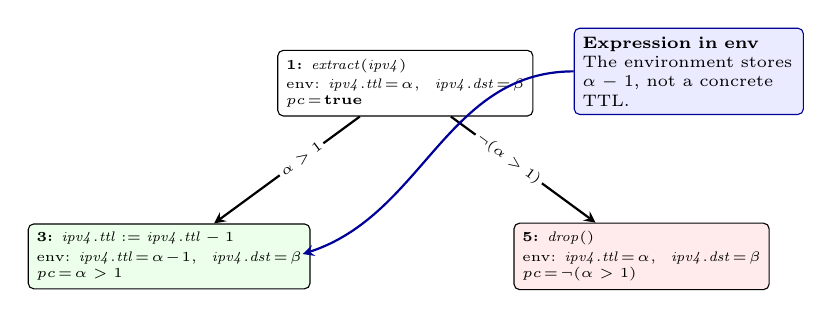
\begin{tikzpicture}[
        >=stealth,
        state/.style={rectangle, draw, rounded corners=2pt,
                     align=left, font=\tiny, inner sep=3pt},
      ]
      % Root: after extract — fields become symbolic
      \node[state] (s1) at (0, 0) {%
        \textbf{1:} $\mathit{extract}(\mathit{ipv4})$\\[1pt]
        env: $\mathit{ipv4.ttl} \!=\! \alpha,\;\; \mathit{ipv4.dst} \!=\! \beta$\\
        $pc \!=\! \mathbf{true}$};

      % T: assignment creates an expression in the env
      \node[state, fill=green!8] (st) at (-3, -2.2) {%
        \textbf{3:} $\mathit{ipv4.ttl} := \mathit{ipv4.ttl} - 1$\\[1pt]
        env: $\mathit{ipv4.ttl} \!=\! \alpha \!-\! 1,\;\; \mathit{ipv4.dst} \!=\! \beta$\\
        $pc \!=\! \alpha > 1$};

      % F: drop, env unchanged, pc accumulated
      \node[state, fill=red!8] (sf) at (3, -2.2) {%
        \textbf{5:} $\mathit{drop}()$\\[1pt]
        env: $\mathit{ipv4.ttl} \!=\! \alpha,\;\; \mathit{ipv4.dst} \!=\! \beta$\\
        $pc \!=\! \neg(\alpha > 1)$};

      % Edges with branch expressions
      \draw[->, thick] (s1) -- node[fill=white, font=\tiny,
        inner sep=1pt, pos=0.4, sloped] {$\alpha > 1$} (st);
      \draw[->, thick] (s1) -- node[fill=white, font=\tiny,
        inner sep=1pt, pos=0.4, sloped] {$\neg(\alpha > 1)$} (sf);

      \only<2->{%
        \node[rectangle, draw=blue!60!black, fill=blue!8, rounded corners=2pt,
          align=left, font=\fontsize{6.2}{7}\selectfont, inner sep=3pt,
          text width=2.7cm] (envnote) at (3.6,0.15) {%
          \textbf{Expression in env}\\
          The environment stores\\
          $\alpha - 1$, not a concrete TTL.};
        \draw[->, blue!60!black, thick]
          (envnote.west) to[out=180,in=18] ($(st.east)+(-0.1,0.03)$);
      }
      \end{tikzpicture}
    \end{column}
  \end{columns}

  \vspace{0.6em}
  \begin{overlayarea}{\textwidth}{3.0cm}
    \begin{enumerate}\setlength\itemsep{3pt}
      \item<2-> \textbf{Symbolic Values:} inputs are replaced by symbols ($\alpha, \beta, \ldots$)
      \item<3-> \textbf{Env:} variables map to \emph{expressions} over symbols, not concrete values
      \item<4-> \textbf{Path Condition ($pc$):} each branch accumulates constraints; the initial path starts with \textbf{true}
      \item<5-> \textbf{Execution Tree:} conditionals \emph{fork} execution into parallel symbolic paths
    \end{enumerate}
  \end{overlayarea}

% Such a tree is a helpful datastructure for verification.
% we can ask, at the end of the program is there a path where the packcet is dropped?
% or we can ask is the packet always dropper or forwarded  
% or we could ask is there any state where tll == 0 or is it true that for all states ttl = 1
\end{frame}









%% Savebox approach: pre-render lstlisting blocks outside the frame
\newsavebox{\pfourheaders}
\begin{lrbox}{\pfourheaders}
\begin{minipage}{0.46\textwidth}
\begin{lstlisting}[style=p4style]
#include <core.p4>
#include <v1model.p4>

header ethernet_t {
    macAddr_t dstAddr;
    macAddr_t srcAddr;
    bit<16>   etherType;
}
header ipv4_t {
    bit<4>    version;
    ...
    ip4Addr_t dstAddr;
}
struct headers {
    ethernet_t ethernet;
    ipv4_t     ipv4;
}
\end{lstlisting}
\end{minipage}
\end{lrbox}

\newsavebox{\pfourparser}
\begin{lrbox}{\pfourparser}
\begin{minipage}{0.46\textwidth}
\begin{lstlisting}[style=p4style]
parser MyParser(packet_in pkt,
    out headers hdr, ...) {
  state start {
    transition parse_ethernet;
  }
  state parse_ethernet {
    pkt.extract(hdr.ethernet);
    transition select(hdr.ethernet.etherType) {
      TYPE_IPV4: parse_ipv4;
      default: accept;
    }
  }
  state parse_ipv4 {
    pkt.extract(hdr.ipv4);
    transition accept;
  }
}
\end{lstlisting}
\end{minipage}
\end{lrbox}

\newsavebox{\pfourcontrol}
\begin{lrbox}{\pfourcontrol}
\begin{minipage}{0.46\textwidth}
\begin{lstlisting}[style=p4style]
control MyIngress(inout headers hdr,
    inout metadata meta, ...) {
  action drop() {
    mark_to_drop(standard_metadata);
  }
  action ipv4_forward(
      macAddr_t dstAddr,
      egressSpec_t port) {
    standard_metadata.egress_spec = port;
    hdr.ethernet.srcAddr =
        hdr.ethernet.dstAddr;
    hdr.ethernet.dstAddr = dstAddr;
    hdr.ipv4.ttl = hdr.ipv4.ttl - 1;
  }
  table ipv4_lpm {
    key = {
      hdr.ipv4.dstAddr: lpm;
    }
    actions = {
      ipv4_forward;
      drop;
      NoAction;
    }
    const entries = {
      32w0x0a000000/8:
        ipv4_forward(48w0x001122334455, 9w1);
    }
    size = 1024;
    default_action = drop();
  }
  apply {
    if (hdr.ipv4.isValid()) {
      ipv4_lpm.apply();
    }
  }
}
\end{lstlisting}
\end{minipage}
\end{lrbox}









\begin{frame}{P4}
\vspace{-0.4cm}
\begin{tikzpicture}
  %% Place code blocks as nodes
  \node[anchor=north west, inner sep=0pt] (headers) at (0,0)
    {\usebox{\pfourheaders}};
  \node[anchor=north west, inner sep=0pt] (parser) at ([yshift=-3pt]headers.south west)
    {\usebox{\pfourparser}};
  \node[anchor=north west, inner sep=0pt] (control) at (0.52\textwidth,0)
    {\usebox{\pfourcontrol}};

  %% Table sub-region (lines 15--26 of ~32 in control block)
  \coordinate (t-nw) at ($(control.north west)!0.44!(control.south west)$);
  \coordinate (t-se) at ($(control.north east)!0.81!(control.south east)$);
  \coordinate (t-actions) at ($(control.north west)!0.66!(control.south west)$);
  \coordinate (t-keyline) at ($(control.north west)!0.50!(control.south west)$);

  %% Progressive overlay highlights (semi-transparent so code shows through)
  \only<1->{%
    \node[fit=(headers), draw=blue!70, thick,
          rounded corners=4pt, inner sep=0pt, text opacity=1] (hbox) {};
    \node[font=\Large\bfseries\sffamily, text=blue!80!black,
          name=hlabel,
          anchor=south, yshift=-2pt] at (hbox.north) {\strut Headers};
  }
  \only<2->{%
    \node[fit=(parser), draw=green!50!black, thick,
          rounded corners=4pt, inner sep=0pt, text opacity=1] (pbox) {};
    \node[font=\Large\bfseries\sffamily, text=green!40!black,
          name=plabel,
          anchor=south, yshift=2pt] at (pbox.south) {\strut Parser};
  }
  \only<3->{%
    \node[fit=(control), draw=violet!70, thick,
          rounded corners=4pt, inner sep=0pt, text opacity=1] (cbox) {};
    \node[font=\Large\bfseries\sffamily, text=violet!80!black,
          name=clabel,
          anchor=south, yshift=-2pt] at (cbox.north) {\strut Control Block};
  }
  \only<4->{%
    \node[fit=(t-nw)(t-se), draw=yellow!70!black, thick,
          rounded corners=4pt, inner sep=0pt, text opacity=1,
          font=\normalsize\bfseries\sffamily, text=yellow!40!black] {Table};
  }
  \only<4>{%
    \node[draw=black!70, fill=white, rounded corners=3pt,
          align=left, font=\fontsize{6.5}{7.3}\selectfont, inner sep=4pt,
          text width=2.9cm, anchor=center] (tnote) at ([xshift=0.9cm]$(headers.north west)!0.5!(parser.south east)$) {%
          Runtime installs rules.\\
          Packet values are compared\\
          against the \texttt{key}.\\
          The matching rule selects\\
          an \texttt{action} to run.};
    \draw[->, thick, black!70] (tnote.east) to[out=0,in=180] ([xshift=0.7cm,yshift=-0.12cm]t-keyline);
    \draw[->, thick, black!70] (tnote.east) to[out=0,in=180] ([xshift=0.9cm]t-actions);
  }
\only<5->{%
    \node[fit=(headers)(parser)(control)(hlabel)(plabel)(clabel),
          fill=white, fill opacity=0.50,
          rounded corners=6pt, inner sep=6pt, draw=none] {};
    \node[draw=black!70, fill=white, rounded corners=4pt,
          text width=0.60\textwidth,
          align=left, font=\footnotesize\sffamily, inner sep=6pt] at
          ($(headers.north west)!0.5!(control.south east)$) {%
          \textbf{Other P4 Domain Features}\par
          \vspace{0.15em}
          \begin{itemize}\setlength\itemsep{2pt}\setlength\parsep{0pt}\setlength\parskip{0pt}\setlength\topsep{2pt}
            \item \textbf{Stateful Objects:} Persist state across multiple packets.
            \begin{itemize}\setlength\itemsep{1pt}\setlength\parsep{0pt}\setlength\parskip{0pt}\setlength\topsep{1pt}
                \item \textbf{Registers:} Mutable read/write memory arrays (used for flow tracking, stateful firewalls, sketches).
                \item \textbf{Counters:} Track packet counts and byte volumes.
                \item \textbf{Meters:} Measure traffic rates and color packets (for QoS and rate limiting).
            \end{itemize}
            \item \textbf{Externs:} Target-specific black-box components (e.g., checksum engines, custom hashers, cryptography).
            \item \textbf{Pipeline / Traffic Management:} Clone/multicast (duplicating packets), recirculate, and digests (sending messages to the control plane).
          \end{itemize}};
  }
  \only<3>{%
    \node[font=\Huge\bfseries\sffamily, text=black] at ($(headers.north west)!0.5!(parser.south east)$) {Syntax};
    \node[font=\Huge\bfseries\sffamily, text=black] at (control.center) {Semantics};
  }
\end{tikzpicture}
\end{frame}


% \begin{frame}{User interaction}
% \centering
% \large Interaction with P4Check happens through generated counterexamples and test inputs.
% \end{frame}

\begin{frame}[fragile]{Grisette}
\vspace{-1cm}
\begin{columns}[T,onlytextwidth]

\begin{column}{0.49\textwidth}
\begin{block}{\centering Concrete}
\begin{lstlisting}[style=haskellstyle, escapeinside={(*}{*)}]
data CExpr = CLit (*\tikz[remember picture,baseline=(ci.base)]\node[inner sep=0pt](ci){Int};*) | CVar String | CBinOp Op CExpr CExpr

data CStmt = CAssign String CExpr | CIf CExpr CStmt CStmt

data CVal  = CInt Int | CBoolVal Bool

type CEnv  = [(String, CVal)]

evalCExpr :: CExpr -> StateT CEnv Identity CVal
evalCExpr (CBinOp op e1 e2) = do
  v1 <- evalCExpr e1; v2 <- evalCExpr e2
  pure $ case (op, v1, v2) of
    (Add, CInt a, CInt b) -> CInt (a + b)
    (Lt,  CInt a, CInt b) -> CBoolVal (a < b)
    _ -> error "Type error"

evalCStmt :: CStmt -> StateT CEnv Identity ()
evalCStmt (CAssign x e) = do
  v <- evalCExpr e; modify (updateCEnv x v)
evalCStmt (CIf cond thenS elseS) = do
  v <- evalCExpr cond
  case v of
    CBoolVal c -> (*\tikz[remember picture,baseline=(cif.base)]\node[inner sep=0pt](cif){if};*) c then evalCStmt thenS else evalCStmt elseS
    _ -> error "Type error"

runConcrete :: CStmt -> CEnv -> CEnv
runConcrete stmt env =
  runIdentity $ execStateT (evalCStmt stmt) env
\end{lstlisting}
\end{block}
\end{column}

\begin{column}{0.49\textwidth}
\begin{block}{\centering Symbolic}
\begin{lstlisting}[style=haskellstyle, escapeinside={(*}{*)}]
data SExpr = SLit (*\tikz[remember picture,baseline=(si.base)]\node[inner sep=0pt](si){SymInteger};*) | SVar String | SBinOp Op SExpr SExpr
  deriving (Generic, Mergeable) via (Default SExpr)
data SStmt = SAssign String SExpr | SIf SExpr SStmt SStmt
  deriving (Generic, Mergeable) via (Default SStmt)
data SVal  = SInt SymInteger | SBoolVal SymBool
  deriving (Generic, Mergeable) via (Default SVal)
type SEnv  = [(String, SVal)]

evalSExpr :: SExpr -> StateT SEnv Union SVal
evalSExpr (SBinOp op e1 e2) = do
  v1 <- evalSExpr e1; v2 <- evalSExpr e2
  mrgReturn $ case (op, v1, v2) of
    (Add, SInt a, SInt b) -> SInt (a + b)
    (Lt,  SInt a, SInt b) -> SBoolVal (a .< b)
    _ -> error "Type error"

evalSStmt :: SStmt -> StateT SEnv Union ()
evalSStmt (SAssign x e) = do
  v <- evalSExpr e; mrgModify (updateSEnv x v)
evalSStmt (SIf cond thenS elseS) = do
  v <- evalSExpr cond
  case v of
    SBoolVal c -> (*\tikz[remember picture,baseline=(sif.base)]\node[inner sep=0pt](sif){mrgIf};*) c (evalSStmt thenS) (evalSStmt elseS)
    _ -> error "Type error"

runSymbolic :: SStmt -> SEnv -> Union SEnv
runSymbolic stmt env =
  execStateT (evalSStmt stmt) env
\end{lstlisting}
\end{block}
\end{column}

\end{columns}
\begin{tikzpicture}[remember picture,overlay]
  \draw[red, thick] (si.center) ellipse (0.7cm and 0.15cm);
  \draw[red, thick] (ci.center) ellipse (0.2cm and 0.15cm);
  \draw[red, thick] (cif.center) ellipse (0.15cm and 0.15cm);
  \draw[red, thick] (sif.center) ellipse (0.35cm and 0.15cm);
  \node[anchor=south east, xshift=-0.5cm, yshift=0.5cm] at (current page.south east) {
    \scriptsize
    \begin{tabular}{r}
      \textbf{Grisette (Ordered Guards):} \\
      $y = \begin{cases}
        a & \text{if } \text{cond}_1 \\
        b & \text{else if } \text{cond}_2 \\
        a & \text{otherwise}
      \end{cases}$
    \end{tabular}
  };
\end{tikzpicture}
\end{frame}
\begin{hidden}
\begin{frame}{P4 Execution}
\centering
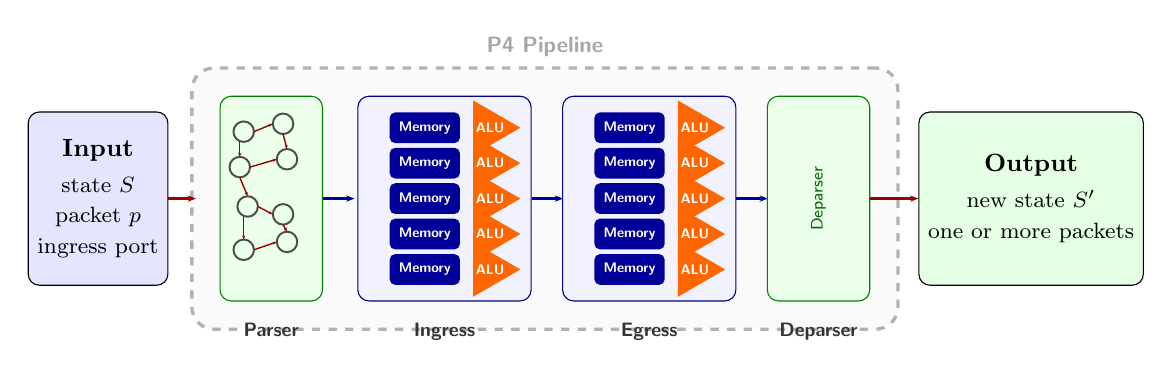
\begin{tikzpicture}[
  x=1cm, y=1cm,
  mem/.style={rectangle, fill=blue!60!black, rounded corners=2pt,
              minimum width=0.85cm, minimum height=0.35cm,
              font=\sffamily\fontsize{5}{6}\selectfont\bfseries, text=white},
  alu/.style={isosceles triangle, isosceles triangle apex angle=60,
              fill=orange!80!red, shape border rotate=0,
              minimum width=0.1cm, minimum height=0.35cm,
              font=\sffamily\fontsize{4.5}{5}\selectfont\bfseries, text=white,
              inner sep=1pt},
  stage/.style={rectangle, draw=blue!50!black, fill=blue!5,
                rounded corners=4pt, inner sep=4pt},
  parserbox/.style={rectangle, draw=green!50!black, fill=green!8,
                    rounded corners=4pt, inner sep=4pt},
  bluearr/.style={-{Stealth[length=3pt]}, blue!60!black, line width=1.2pt},
  redarr/.style={-{Stealth[length=3pt]}, red!60!black, line width=1.2pt},
  lbl/.style={font=\sffamily\fontsize{7}{8}\selectfont\bfseries, text=black!80},
]

%% ===== INPUT BOX =====
\node[rectangle, draw, rounded corners=4pt, fill=blue!10,
      minimum height=2.2cm, minimum width=1.6cm, align=center, font=\small]
  (input) at (-1.2,0) {
  \textbf{Input}\\[2pt]
  \footnotesize state $S$\\
  \footnotesize packet $p$\\
  \footnotesize ingress port
};

%% ===== Arrow: Input -> Parser =====
\draw[redarr] (input.east) -- ++(0.35,0);

%% ===== PARSER =====
\node[parserbox, minimum width=1.3cm, minimum height=2.6cm] (parser) at (1.0,0) {};
% Parse-graph nodes
\foreach \cx/\cy in {0.65/0.85, 1.15/0.95, 0.6/0.4, 1.2/0.5,
                      0.7/-0.1, 1.15/-0.2, 0.65/-0.65, 1.2/-0.55} {
  \draw[black!70, line width=0.7pt] (\cx,\cy) circle (0.13cm);
}
% Parse-graph edges
\foreach \ax/\ay/\bx/\by in {
  0.78/0.85/1.02/0.95, 1.15/0.82/1.2/0.63,
  0.6/0.72/0.6/0.53, 0.73/0.4/1.07/0.5,
  0.6/0.27/0.7/0.03, 0.83/-0.1/1.02/-0.2,
  1.15/-0.33/1.2/-0.42, 0.65/-0.23/0.65/-0.52,
  0.78/-0.65/1.07/-0.55} {
  \draw[-{Stealth[length=1.5pt]}, red!60!black, line width=0.5pt]
    (\ax,\ay) -- (\bx,\by);
}
\node[lbl, below] at (1.0,-1.45) {Parser};

%% ===== ARROW: Parser -> Ingress =====
\draw[bluearr] (parser.east) -- ++(0.4,0);

%% ===== INGRESS =====
\node[stage, minimum width=2.2cm, minimum height=2.6cm] (ingress) at (3.2,0) {};
\foreach \row in {0.9, 0.45, 0.0, -0.45, -0.9} {
  \node[mem] at (2.95, \row) {Memory};
  \node[alu] at (3.78, \row) {ALU};
}
\node[lbl, below] at (3.2,-1.45) {Ingress};

%% ===== ARROW: Ingress -> Egress =====
\draw[bluearr] (ingress.east) -- ++(0.4,0);

%% ===== EGRESS =====
\node[stage, minimum width=2.2cm, minimum height=2.6cm] (egress) at (5.8,0) {};
\foreach \row in {0.9, 0.45, 0.0, -0.45, -0.9} {
  \node[mem] at (5.55, \row) {Memory};
  \node[alu] at (6.38, \row) {ALU};
}
\node[lbl, below] at (5.8,-1.45) {Egress};

%% ===== ARROW: Egress -> Deparser =====
\draw[bluearr] (egress.east) -- ++(0.4,0);

%% ===== Deparser =====
\node[parserbox, minimum width=1.3cm, minimum height=2.6cm] (deparser) at (7.95,0) {};
\node[font=\sffamily\fontsize{6}{7}\selectfont, text=green!40!black, rotate=90]
  at (7.95,0) {Deparser};
\node[lbl, below] at (7.95,-1.45) {Deparser};

%% ===== PIPELINE OUTLINE =====
\begin{scope}[on background layer]
  \node[draw=gray!60, dashed, line width=1.2pt, rounded corners=8pt,
        fill=gray!4, inner sep=10pt, fit=(parser)(ingress)(egress)(deparser),
        label={[font=\sffamily\footnotesize\bfseries, text=gray!70]above:P4 Pipeline}] (pipeline) {};
\end{scope}

%% ===== OUTPUT BOX =====
\node[rectangle, draw, rounded corners=4pt, fill=green!10,
      minimum height=2.2cm, minimum width=1.8cm, align=center, font=\small]
  (output) at (10.65,0) {
  \textbf{Output}\\[2pt]
  \footnotesize new state $S'$\\
  \footnotesize one or more packets
};

%% ===== Arrow: Pipeline -> Output =====
\draw[redarr] (deparser.east) -- (output.west);

\end{tikzpicture}

\bigskip
\begin{columns}[T]
\begin{column}{0.48\textwidth}
\small
\textbf{Semantics of processing one packet:}
\[
  (S,\; p,\; \mathit{port}) \;\longrightarrow\; (S',\; \{\mathcal{M}(p_i, \mathit{port}_i)\})
\]
A single packet produces a \emph{multiset} of (packet, output port) pairs
\end{column}

\begin{column}{0.48\textwidth}
\small
\textbf{Clone \& Multicast:}
\begin{itemize}\setlength\itemsep{3pt}
  \item \textbf{Clone:} duplicates a packet mid-pipeline (e.g.\ \texttt{clone3}). The original continues normally
  \item \textbf{Multicast:} the ingress sets a \texttt{mcast\_grp}; One input packet $\to$ many output pairs.
\end{itemize}
\end{column}
\end{columns}
\end{frame}
\end{hidden}


\begin{frame}
\centering
\includesvg[width=\textwidth,height=0.82\textheight,keepaspectratio]{p4checkarch.drawio.svg}
\end{frame}



\section{Problem \& Scope}
\begin{hidden}
\begin{frame}{Verification Properties: Three Levels}
\centering
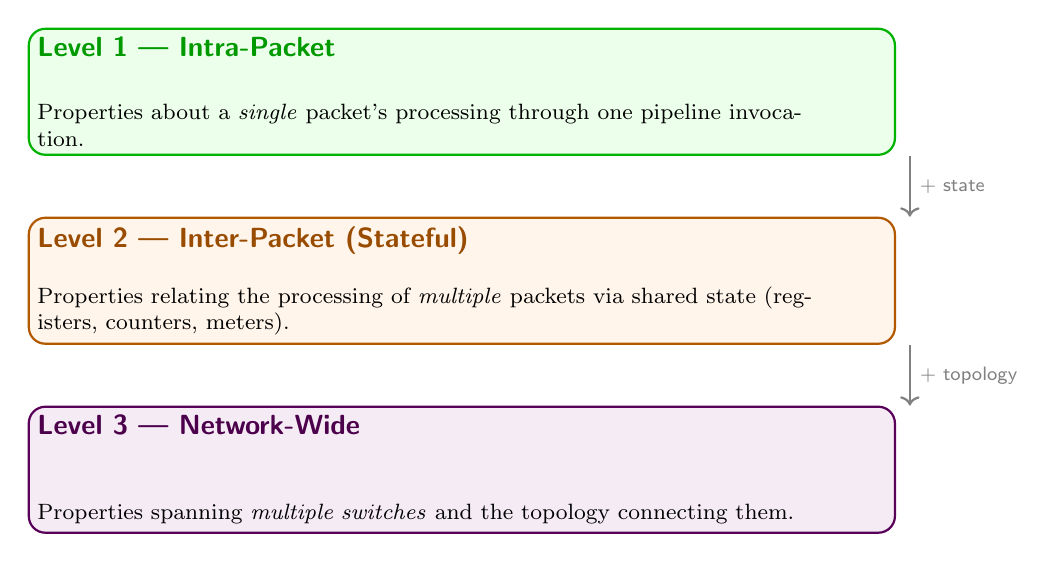
\begin{tikzpicture}

\node[rectangle, rounded corners=6pt, draw=green!70!black, thick,
      fill=green!8, minimum width=11cm, minimum height=1.6cm,
      text=black, font=\small, align=left, inner sep=10pt] (L1) at (0, 2.4) {};
\node[anchor=north west, font=\bfseries\sffamily\normalsize, text=green!60!black]
  at (L1.north west) {Level 1 --- Intra-Packet};
\node[anchor=south west, font=\footnotesize, text width=10cm] at (L1.south west)
  {Properties about a \emph{single} packet's processing through one pipeline invocation.};

\node[rectangle, rounded corners=6pt, draw=orange!70!black, thick,
      fill=orange!8, minimum width=11cm, minimum height=1.6cm,
      text=black, font=\small, align=left, inner sep=10pt] (L2) at (0, 0) {};
\node[anchor=north west, font=\bfseries\sffamily\normalsize, text=orange!60!black]
  at (L2.north west) {Level 2 --- Inter-Packet (Stateful)};
\node[anchor=south west, font=\footnotesize, text width=10cm] at (L2.south west)
  {Properties relating the processing of \emph{multiple} packets via shared state (registers, counters, meters).};

\node[rectangle, rounded corners=6pt, draw=violet!70!black, thick,
      fill=violet!8, minimum width=11cm, minimum height=1.6cm,
      text=black, font=\small, align=left, inner sep=10pt] (L3) at (0, -2.4) {};
\node[anchor=north west, font=\bfseries\sffamily\normalsize, text=violet!60!black]
  at (L3.north west) {Level 3 --- Network-Wide};
\node[anchor=south west, font=\footnotesize, text width=10cm] at (L3.south west)
  {Properties spanning \emph{multiple switches} and the topology connecting them.};

% Arrows on the right showing increasing scope
\draw[->, thick, gray] ([xshift=5pt]L1.south east) -- ([xshift=5pt]L2.north east)
  node[midway, right, font=\scriptsize\sffamily, text=gray] {+ state};
\draw[->, thick, gray] ([xshift=5pt]L2.south east) -- ([xshift=5pt]L3.north east)
  node[midway, right, font=\scriptsize\sffamily, text=gray] {+ topology};

\end{tikzpicture}
\end{frame}
\end{hidden}

\begin{frame}{Verification Properties: Three Levels -- Examples}
\begin{columns}[T,onlytextwidth]
  \begin{column}{0.54\textwidth}
    \centering
    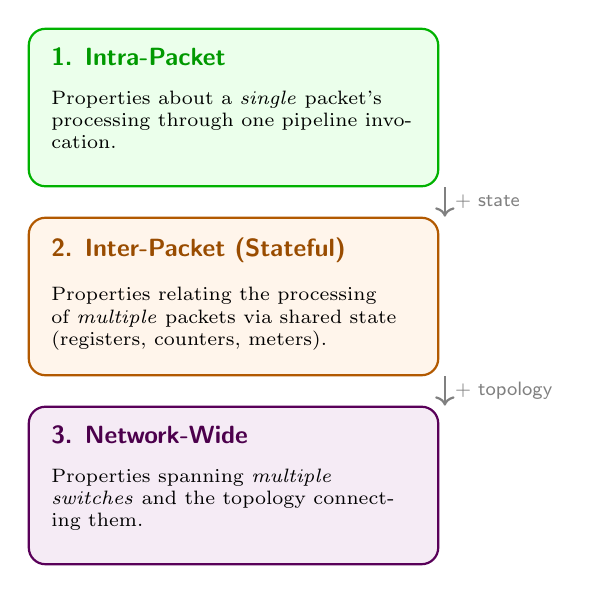
\begin{tikzpicture}

    \node[rectangle, rounded corners=6pt, draw=green!70!black, thick,
          fill=green!8, minimum width=5.2cm, minimum height=2.0cm,
          text=black, font=\scriptsize, align=left, inner sep=6pt] (L1) at (0, 2.4) {};
    \node[anchor=north west, font=\bfseries\sffamily\small, text=green!60!black]
      (L1T) at ([shift={(5pt,-4pt)}]L1.north west) {1. Intra-Packet};
    \node[anchor=north west, font=\scriptsize, text width=4.6cm] at ([shift={(0,-2pt)}]L1T.south west)
      {Properties about a \emph{single} packet's processing through one pipeline invocation.};

    \node[rectangle, rounded corners=6pt, draw=orange!70!black, thick,
          fill=orange!8, minimum width=5.2cm, minimum height=2.0cm,
          text=black, font=\scriptsize, align=left, inner sep=6pt] (L2) at (0, 0) {};
    \node[anchor=north west, font=\bfseries\sffamily\small, text=orange!60!black]
      (L2T) at ([shift={(5pt,-4pt)}]L2.north west) {2. Inter-Packet (Stateful)};
    \node[anchor=north west, font=\scriptsize, text width=4.6cm] at ([shift={(0,-2pt)}]L2T.south west)
      {Properties relating the processing of \emph{multiple} packets via shared state (registers, counters, meters).};

    \node[rectangle, rounded corners=6pt, draw=violet!70!black, thick,
          fill=violet!8, minimum width=5.2cm, minimum height=2.0cm,
          text=black, font=\scriptsize, align=left, inner sep=6pt] (L3) at (0, -2.4) {};
    \node[anchor=north west, font=\bfseries\sffamily\small, text=violet!60!black]
      (L3T) at ([shift={(5pt,-4pt)}]L3.north west) {3. Network-Wide};
    \node[anchor=north west, font=\scriptsize, text width=4.6cm] at ([shift={(0,-2pt)}]L3T.south west)
      {Properties spanning \emph{multiple switches} and the topology connecting them.};

    \draw[->, thick, gray] ([xshift=2pt]L1.south east) -- ([xshift=2pt]L2.north east)
      node[midway, right, font=\scriptsize\sffamily, text=gray] {+ state};
    \draw[->, thick, gray] ([xshift=2pt]L2.south east) -- ([xshift=2pt]L3.north east)
      node[midway, right, font=\scriptsize\sffamily, text=gray] {+ topology};

    \end{tikzpicture}
  \end{column}

  \begin{column}{0.42\textwidth}
    \hspace*{-0.5cm}%
    \begin{minipage}{\dimexpr\linewidth+0.5cm\relax}
    \begin{itemize}
      \item \textbf{\small 1. Examples:}
        \begin{itemize}\setlength\itemsep{4pt}
          \item \scriptsize If \texttt{ipv4.ttl == 0} at ingress, packet is always dropped.
                \\ \textcolor{teal}{\texttt{if hdr.ipv4.ttl@Ingress.start == 0 then hit@drop}}
          \item \scriptsize Every path through ingress either drops or sets \texttt{egress\_spec}.
                \\ \textcolor{teal}{\texttt{hit@drop || eg\_spec@Ingress.end != 9w511}}
        \end{itemize}

      \item \textbf{\small 2. CTL with intra-packet as atom}
        \begin{itemize} % Trace is the sequence of register states
          \item \scriptsize Reachability: From any starting state, it is possible for \texttt{r[4]} to eventually reach value.
        \end{itemize}

      \item \textbf{\small 3. Examples:}
        \begin{itemize} % state is sequence of idk exactly 
          \item \scriptsize Pkt entering \texttt{s1} on \texttt{p1} in prefix $P$ reaches \texttt{s5} on \texttt{p3}.
        \end{itemize}
    \end{itemize}
    \end{minipage}
  \end{column}
\end{columns}
\end{frame}


% ────────────────────────────────────────────────────────────
%  LEVEL 1 — INTRA-PACKET
% ────────────────────────────────────────────────────────────

% % Grammar
% \begin{frame}{Level 1: Intra-Packet Properties}
% Properties about a \textbf{single packet} processed through \textbf{one pipeline invocation}.
% Asserstions with pre and postconditions realting different prorgram components 

% grammar:
% \mathit{location} ::=~&~ name(x) && (\text{control or action})\\
%     |~&~ start ~|~ end  \\[6pt]
% %
% \mathit{spec} ::=~& \mathbf{if}\ \mathit{spec}\ \mathbf{then}\ \mathit{spec}\ \mathbf{else}\ \mathit{spec}? && {\text{(intra packet)}} \\ 
%                  |~& \mathit{expr} @ \mathit{location}\\
%                  |~& \mathit{hit} @ \mathit{location}\\ && (\text{Reachability of a location})
%                  |~& \mathit{const} \\
%                  |~& \mathit{spec} \oplus \mathit{spec} && {\text{Normal P4 operators }}
%                  \\[6pt]



%                  \begin{frame}
% {Ghost variable instrumentation}

% Conceptually: Check that specification evaluates to true on all leaf branches 
% \end{frame}

% \end{frame}
\begin{frame}{Level 1: Intra-Packet Properties}
  Properties about a \textbf{single packet} processed through \textbf{one pipeline invocation}.\\
  Assertions with pre- and post-conditions relating different program components.

  \vspace{0.5em}
  \begin{block}{Specification Grammar}
    \small
    \vspace{-1.5em}
    \begin{align*}
      \mathit{loc} \quad &::= \quad \mathit{name}(x) \mid \mathit{start} \mid \mathit{end} && \text{\footnotesize (Control or action boundaries)} \\[4pt]
      \mathit{spec} \quad &::= \quad \mathbf{if}\ \mathit{spec}\ \mathbf{then}\ \mathit{spec}\ [\mathbf{else}\ \mathit{spec}] && \text{\footnotesize (Intra-packet implication)} \\
                          &\mid \quad \mathit{expr} \mathop{@} \mathit{loc} && \text{\footnotesize (Value at a specific location)} \\
                          &\mid \quad \mathit{hit} \mathop{@} \mathit{loc} && \text{\footnotesize (Reachability of a location)} \\
                          &\mid \quad \mathit{const} \quad\mid\quad \mathit{spec} \oplus \mathit{spec} && \text{\footnotesize (Constants and standard P4 operators)}
    \end{align*}
  \end{block}

  \vspace{0.1em}
  \textbf{Example:} \texttt{hdr.ipv4.ttl@Ingress.start}

  \vspace{0.5em}
  \begin{block}{Ghost Variable Instrumentation}
    \small
    \textbf{Conceptually:} Check that the specification evaluates to \textbf{true} on all execution leaf branches.
  \end{block}
\end{frame}
% Examples

% \begin{frame}{Level 1: Intra-Packet Properties}
% \small
% % Properties about a \textbf{single packet} processed through \textbf{one pipeline invocation}.
% % \textbf{quantified over state and table configs}
% % \medskip
% \begin{enumerate}

%   \item If \texttt{ipv4.ttl == 0} at ingress entry, the packet is always dropped.
%         \only<2>{\hfill  \textcolor{teal}{[if ipv4.tll@Ingress.start == 0 then drop@Egress.end ]}}

%         % This one is not super relevant for bmv2
%   % \item A packet is never both dropped \emph{and} forwarded to an egress port.
%   %       \only<2>{\hfill \textcolor{teal}{[formula]}}
%   % !({standard_metadata.egress_spec @ MyIngress.end == 9w511}
%                     %  && {standard_metadata.egress_spec @ MyIngress.end != 9w511}

%                     % This same mechanism can be used to specify a single action 
%   \item The TTL field is decremented by exactly one if the packet is forwarded.
%         \only<2>{\hfill  \textcolor{teal}{[if standard_metadata.egress_spec @ MyIngress.end != 9w511
%                then hdr.ipv4.ttl @ MyIngress.end == hdr.ipv4.ttl @ MyIngress.begin - 8w1}]}}

%   \item \texttt{hdr.ethernet.etherType} is never modified by the ingress control.
%         \only<2>{\hfill  \textcolor{teal}{[hdr.ethernet.etherType @ MyIngress.end ==
%                            hdr.ethernet.etherType @ MyIngress.begin]}}

%   \item[\textbf{Control-flow / path}]
%   \item If action \texttt{ipv4\_forward} is hit, then \texttt{egress\_spec} is set to a non-drop value.
%         \only<2>{\hfill  \textcolor{teal}{[formula]}}

%   \item Every path through ingress either drops the packet or sets \texttt{egress\_spec}.
%         \only<2>{\hfill \textcolor{teal}{[formula]}}

%   \item Two actions $x,y$ are mutually exclusive
%         \only<2>{\hfill  \textcolor{teal}{[formula]}}

% \item There is no path where \texttt{mark\_to\_drop()} is called and then \texttt{egress\_spec} is subsequently overwritten.
%         \only<2>{\hfill  \textcolor{teal}{[cant be expressed ]}}
% \end{enumerate}
% \end{frame}

\begin{hidden}
\begin{frame}{Level 1: Intra-Packet Examples}
\small
\begin{enumerate}
  \only<1>{\setlength\itemsep{8pt}}
  \only<2->{\setlength\itemsep{1pt}}

  \item If \texttt{ipv4.ttl == 0} at ingress entry, the packet is always dropped.
        \only<2->{\\ \textcolor{teal}{\texttt{if hdr.ipv4.ttl @ Ingress.start == 0 then hit @ drop}}}

  \item The TTL field is decremented by exactly one if the packet is forwarded.
        \only<2->{\\ \textcolor{teal}{\texttt{if standard\_metadata.egress\_spec @ Ingress.end != 9w511 \\
        \hspace*{1.5em} then hdr.ipv4.ttl @ Ingress.end == hdr.ipv4.ttl @ Ingress.start - 8w1}}}

  \item \texttt{hdr.ethernet.etherType} is never modified by the ingress control.
        \only<2->{\\ \textcolor{teal}{\texttt{hdr.ethernet.etherType @ Ingress.end == hdr.ethernet.etherType @ Ingress.start}}}
  
  \item If action \texttt{ipv4\_forward} is hit, then \texttt{egress\_spec} is set to a non-drop value.
        \only<2->{\\ \textcolor{teal}{\texttt{if hit @ ipv4\_forward then standard\_metadata.egress\_spec @ Ingress.end != 9w511}}}

  \item Every path through ingress either drops the packet or sets \texttt{egress\_spec}.
        \only<2->{\\ \textcolor{teal}{\texttt{hit @ drop || standard\_metadata.egress\_spec @ Ingress.end != 9w511}}}

  \item Two actions $x$ and $y$ are mutually exclusive.
        \only<2->{\\ \textcolor{teal}{\texttt{!(hit @ x \&\& hit @ y)}}}

  \item \textbf{Limitation:} There is no path where \texttt{mark\_to\_drop()} is called and \texttt{egress\_spec} is subsequently overwritten.
        \only<2->{\\ \textcolor{red!70!black}{\textit{[Cannot be expressed: requires temporal reasoning within the pipeline]}}}

\end{enumerate}
\end{frame}
\end{hidden}

% ────────────────────────────────────────────────────────────
%  LEVEL 2 — INTER-PACKET (STATEFUL)
% ────────────────────────────────────────────────────────────
\begin{hidden}
\begin{frame}{Level 2: Inter-Packet (Stateful) Properties}
\small
Properties relating the processing of \textbf{multiple packets} through shared mutable state
(registers, counters, meters, digest/clone sessions).

\medskip
\begin{enumerate}

\item Mutual exclusion: Two registers are never simultaneously nonzero
  \item If register \texttt{blocked[h]} is set to 1 for some source IP \texttt{h}, then \emph{all subsequent} packets from \texttt{h} are dropped.

  \item Persistence: Once register r[4] takes value 5, it holds 5 forever.

   \item Reachability: From any starting state, it is possible for r[4] to eventually reach value 5.

\end{enumerate}
\end{frame}
\end{hidden}


% ────────────────────────────────────────────────────────────
%  LEVEL 3 — NETWORK-WIDE
% ────────────────────────────────────────────────────────────
\begin{hidden}
\begin{frame}{Level 3: Network-Wide Properties}
\small
Properties spanning \textbf{multiple switches} connected by a topology.
Requires reasoning about forwarding across hops.

\medskip
\begin{enumerate}

  \item[\textbf{Reachability}]
  \item Every packet entering switch $s_1$ on port 1 with destination IP in prefix $P$ eventually reaches switch $s_5$ on port 3.
  \item Host $A$ can reach host $B$ if and only if host $B$ can reach host $A$ (symmetry).

  \item[\textbf{Loop freedom}]
  \item No packet visits the same switch twice (loop-free forwarding).

\end{enumerate}
\end{frame}
\end{hidden}

% \begin{frame}{Validation: Did we implement P4?}
% \begin{itemize}
% Concrete Path: generate input + expected output pairs for ech control flow path using p4testgen -> does the concrete interpreter provide the same output 
% Symbolic Path: again using p4testgen, solve for a a given input, is the p4 testgen expected output the only possible packet 

% Generate input output pairs from symbolic -> run with hol4p4 interpreter 
% \end{itemize}
% \end{frame}

\begin{frame}{}
\centering
\Huge
Demo
\end{frame}

\begin{frame}{Testing: Did we implement P4?}
  \begin{itemize}
    \item Concrete Interpreter: P4TestGen-generated input output pairs, check output is the same. \\
    68 real programs: 
    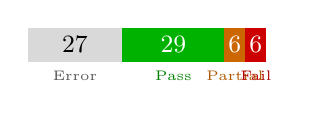
\begin{tikzpicture}[x=0.25\textwidth, y=1.2em, baseline=0.2em]
      \fill[gray!30] (0,0) rectangle (0.397,1);
      \node at (0.198, 0.5) {\small 27};
      \fill[green!70!black] (0.397,0) rectangle (0.824,1) node[pos=.5, white] {\small 29};
      \fill[orange!80!black] (0.824,0) rectangle (0.912,1) node[pos=.5, white] {\small 6};
      \fill[red!80!black] (0.912,0) rectangle (1,1) node[pos=.5, white] {\small 6};

      \node[anchor=north, gray!70!black] at (0.198,0) {\tiny Error};
      \node[anchor=north, green!50!black] at (0.611,0) {\tiny Pass};
      \node[anchor=north, orange!70!black] at (0.868,0) {\tiny Partial};
      \node[anchor=north, red!70!black] at (0.956,0) {\tiny Fail};
    \end{tikzpicture}

    \\[1.4em]
    p4c programs:
    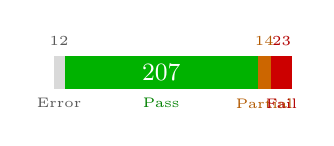
\begin{tikzpicture}[x=0.25\textwidth, y=1.2em, baseline=0.2em]
      \fill[gray!30] (0,0) rectangle (0.047,1);
      \fill[green!70!black] (0.047,0) rectangle (0.855,1) node[pos=.5, white] {\small 207};
      \fill[orange!80!black] (0.855,0) rectangle (0.910,1);
      \fill[red!80!black] (0.910,0) rectangle (1,1);

      \node[anchor=south, gray!70!black] at (0.023,1) {\tiny 12};
      \node[anchor=south, orange!70!black] at (0.883,1) {\tiny 14};
      \node[anchor=south, red!70!black] at (0.955,1) {\tiny 23};

      \node[anchor=north, gray!70!black] at (0.023,0) {\tiny Error};
      \node[anchor=north, green!50!black] at (0.451,0) {\tiny Pass};
      \node[anchor=north, orange!70!black] at (0.883,0) {\tiny Partial};
      \node[anchor=north, red!70!black] at (0.955,0) {\tiny Fail};
    \end{tikzpicture}    \item Symbolic Interpreter (Ongoing): For a spec that instruments such that we select the execution that corresponds to a P4TestGen-generated input, is the expected output included among the possible outcomes (as allowed by the overapproximation)?
  \end{itemize}
\end{frame}

\begin{frame}{Conclusion}
  \begin{columns}[T]
    
    \begin{column}{0.48\textwidth}
    %   \begin{block}{Summary}
        \begin{itemize}
          \item Leverage \textbf{Grisette}: Concrete and Symbolic execution from a mostly shared codebase.
          \item Goal: model the full range of P4 and Architecture features
          \item Verification at program and network level
    %       \item \textbf{Model in Haskell:} Robust implementation supporting the full range of P4 features (parsers, tables, stateful objects).
    %       \item \textbf{Architecture Support:} Accurately models target-specific backends, including \textbf{Tofino (TNA)}, V1Model, and PSA.
    %       \item \textbf{Versatile Verification:} Enables finding invalid accesses and checking user-specified assertions across multiple packets.
        \end{itemize}
      % \end{block}
    \end{column}
    
    \begin{column}{0.48\textwidth}
      \begin{block}{Future work}
        \begin{itemize}\setlength\itemsep{6pt}
          \item Synthesis for program repair
          \item Equivalence checking
          \item NetKAT as a specification language
          \item Control plane model
        \end{itemize}
      \end{block}
    \end{column}
    
  \end{columns}
\end{frame}

\begin{hidden}

\begin{frame}{Conclusion}
  \begin{columns}[T]
    
    % Left Column: Summary of the talk
    \begin{column}{0.48\textwidth}
      \begin{block}{Summary}
        \small
        \begin{itemize}\setlength\itemsep{6pt}
          \item \textbf{Unified Engine:} Concrete and symbolic execution from a single Grisette codebase.
          \item \textbf{ Verification:} properties across three levels:
          \begin{enumerate}\setlength\itemsep{2pt}
              \item \textit{Intra-packet} (via ghost variables)
              \item \textit{Inter-packet} (stateful multi-packet)
              \item \textit{Network-wide}
          \end{enumerate}
          % \item \textbf{Accurate Packet Model:} Novel \textit{construction list} approach gracefully handles arbitrary-length symbolic payloads and lookaheads.
        \end{itemize}
      \end{block}
    \end{column}
    
    % Right Column: Future Work
    \begin{column}{0.48\textwidth}
      \begin{block}{Future Work}
        \small
        \begin{itemize}\setlength\itemsep{8pt}
          \item \textbf{NetKAT Integration:}\\
                NetKAT (and its stateful variants) as a higher-level specification language to express network-wide routing and reachability policies.
          \item \textbf{Control-Plane Co-verification:}\\
                Incorporate dynamic table-rule updates to reason about control-plane and data-plane interactions.
        \end{itemize}
      \end{block}
    \end{column}
    
  \end{columns}
\end{frame}


\begin{frame}[allowframebreaks]{References}
  \scriptsize
  \printbibliography[heading=none]
\end{frame}



% \begin{frame}{Syntax of $\Pi4$}
% \begin{columns}[T]

% %% Left column: grammar (progressive reveal)
% \begin{column}{0.55\textwidth}
% \small
% \begin{align*}
% \uncover<2->{\tau \quad &::= \quad \varnothing \mid \top \mid \Sigma x : \tau.\tau \mid \tau + \tau \mid \{x : \tau \mid \varphi\} \mid \tau[x \mapsto \tau] \\}
% \uncover<3->{\sigma \quad &::= \quad \mathbb{N} \mid \mathbb{B} \mid \mathrm{BV} \mid (x : \tau) \to \tau \\}
% \uncover<4->{\varphi \quad &::= \quad e = e \mid e > e \mid \varphi \land \varphi \mid \neg\varphi \mid x.\iota.\mathit{valid} \mid \mathbf{true} \mid \mathbf{false} \\}
% \uncover<5->{e \quad &::= \quad n \mid \mathit{bv} \mid |x.p| \mid e + e \mid e\mathop{@}e \mid x.p \mid x.p[l\!:\!r] \mid x.\iota[l\!:\!r] \\}
% \uncover<6->{\mathit{bv} \quad &::= \quad \langle\rangle \mid 0 :: \mathit{bv} \mid 1 :: \mathit{bv} \mid \mathrm{b_n} :: \mathit{bv} \\}
% \uncover<7->{p \quad &::= \quad \mathit{pkt_{in}} \mid \mathit{pkt_{out}} \\}
% \uncover<8->{c \quad &::= \quad \mathit{extract}(\iota) \mid \mathit{if}\,(\varphi)\ c\ \mathit{else}\ c \mid c;\, c \mid \iota.f := e \mid \mathit{remit}(\iota) \\}
% \uncover<8->{&\quad\phantom{::=}\quad \mathit{skip} \mid \underline{\mathit{reset}} \mid \mathit{add}(\iota) \mid c\ \mathit{as}\ (x : \tau) \to \tau \\}
% \uncover<9->{d \quad &::= \quad \eta\ \{\overline{f : \mathrm{BV}}\} \mid \iota \mapsto \eta \\}
% \uncover<10->{P \quad &::= \quad (\overline{d}, c)}
% \end{align*}
% \end{column}

% %% Right column: explanations (each replaces the previous)
% \begin{column}{0.42\textwidth}
% \footnotesize

% \only<2>{%
% \textbf{Heap types ($\tau$)}

% \medskip
% Sets of possible packet heaps.
% \begin{itemize}\setlength\itemsep{0.2em}
%   \item $\varnothing$ = empty (impossible state)
%   \item $\top$ = any heap (top type)
%   \item $\Sigma$ = dependent concatenation
%   \item $+$ = union (branching paths)
%   \item $\{x:\tau\mid\varphi\}$ = refinement with predicate
%   \item $\tau[x\mapsto\tau]$ = substitution
% \end{itemize}
% }

% \only<3>{%
% \textbf{Base types ($\sigma$)}

% \medskip
% Primitive types:
% \begin{itemize}\setlength\itemsep{0.2em}
%   \item $\mathbb{N}$ = naturals
%   \item $\mathbb{B}$ = booleans
%   \item $\mathrm{BV}$ = bit vectors
% \end{itemize}

% \medskip
% Commands typed as heap transformers:
% \begin{itemize}
%   \item $(x:\tau)\to\tau$ maps input heap to output heap
% \end{itemize}
% }

% \only<4>{%
% \textbf{Formulae ($\varphi$)}

% \medskip
% Boolean predicates over expressions.
% \begin{itemize}\setlength\itemsep{0.2em}
%   \item $e = e$, $e > e$ --- comparisons
%   \item $\varphi \land \varphi$, $\neg\varphi$ --- logical connectives
%   \item $x.\iota.\mathit{valid}$ --- checks header instance validity
%   \item $\mathbf{true}$, $\mathbf{false}$ --- constants
% \end{itemize}

% \medskip
% Key: validity checks enable safe packet access.
% }

% \only<5>{%
% \textbf{Expressions ($e$)}

% \medskip
% Values that appear in predicates.
% \begin{itemize}\setlength\itemsep{0.2em}
%   \item $n$, $\mathit{bv}$ --- literal numbers and bit vectors
%   \item $|x.p|$ = packet length
%   \item $e + e$ = addition
%   \item $e\mathop{@}e$ = bit concatenation
%   \item $x.p$ = packet access
%   \item $x.p[l\!:\!r]$, $x.\iota[l\!:\!r]$ = bit slicing
% \end{itemize}
% }

% \only<6>{%
% \textbf{Bit vectors ($\mathit{bv}$)}

% \medskip
% List-like encoding of bit strings.
% \begin{itemize}\setlength\itemsep{0.2em}
%   \item $\langle\rangle$ = empty bit vector
%   \item $0 :: \mathit{bv}$ = cons with bit 0
%   \item $1 :: \mathit{bv}$ = cons with bit 1
%   \item $\mathrm{b_n} :: \mathit{bv}$ = cons with symbolic bit variable
% \end{itemize}
% }

% \only<7>{%
% \textbf{Packets ($p$)}

% \medskip
% Two packet buffers:
% \begin{itemize}\setlength\itemsep{0.2em}
%   \item $\mathit{pkt_{in}}$ --- incoming packet (consumed during parsing)
%   \item $\mathit{pkt_{out}}$ --- outgoing packet (built during deparsing)
% \end{itemize}
% }

% \only<8>{%
% \textbf{Commands ($c$)}

% \medskip
% P4 operations:
% \begin{itemize}\setlength\itemsep{0.2em}
%   \item $\mathit{extract}(\iota)$ --- parse header from packet
%   \item $\mathit{if}\,(\varphi)\ c\ \mathit{else}\ c$ --- conditional
%   \item $c;\, c$ --- sequential composition
%   \item $\iota.f := e$ --- field assignment
%   \item $\mathit{remit}(\iota)$ --- serialize header to packet
%   \item $\mathit{skip}$ --- no-op
%   \item $\underline{\mathit{reset}}$ --- pipeline stage boundary
%   \item $\mathit{add}(\iota)$ --- create header instance
%   \item $c\ \mathit{as}\ (x:\tau)\to\tau$ --- type ascription
% \end{itemize}
% }

% \only<9>{%
% \textbf{Declarations ($d$)}

% \medskip
% Define the header structure:
% \begin{itemize}\setlength\itemsep{0.2em}
%   \item $\eta\ \{\overline{f : \mathrm{BV}}\}$ --- header type with named bit-vector fields
%   \item $\iota \mapsto \eta$ --- bind instance name to header type
% \end{itemize}
% }

% \only<10>{%
% \textbf{Programs ($P$)}

% \medskip
% A complete $\Pi4$ program:
% \begin{itemize}\setlength\itemsep{0.2em}
%   \item A sequence of declarations ($\overline{d}$)
%   \item Followed by a command ($c$)
% \end{itemize}

% \medskip
% Declarations define header types and instances; the command processes packets.
% }

% \end{column}
% \end{columns}
% \end{frame}



% \begin{frame}{Level}
% \begin{enumerate}
% \item Intra-packet: at any point during the execution $x == 5$ 
%   at all programs ends $x == 5$, or at some program end
%   if function foo is executed then eventually function y is exectuted 
% \item Inter Packet 
%     if during the processing of some packet the ohnoddos function is exectued then for all fututr pakcet if the ipv4 adress is the same the packet is dropped
% \item Network: 
%   if in switch1 program1 a packet hits action foo then next the packet is processed by switch 2 or eventually the program is proccessed by switch 5 
% \end{enumerate}
% \end{frame}



% \begin{frame}{NetKat}
% Kleene algebra with tests, for networks

% Many many variants
% \end{frame}

% \begin{frame}{NetKAT Syntax}
% \begin{columns}[T]

% %% Left column: NetKAT grammar (progressive reveal)
% \begin{column}{0.48\textwidth}
% \small
% \begin{align*}
% \uncover<1->{\text{Fields} \quad f \quad &::= \quad f_1 \mid \cdots \mid f_k \\}
% \uncover<2->{\text{Packets} \quad pk \quad &::= \quad \{f_1 \!=\! v_1, \cdots, f_k \!=\! v_k\} \\}
% \uncover<3->{\text{Histories} \quad h \quad &::= \quad pk::\langle\rangle \mid pk::h \\}
% \uncover<4->{\text{Predicates} \quad a, b \quad &::= \quad 1 \mid 0 \mid f = n \\ 
% &\quad\phantom{::=}\quad \mid a + b \mid a \cdot b \mid \neg a \\}
% \uncover<5->{\text{Policies} \quad p, q \quad &::= \quad a \mid f \leftarrow n \mid p + q \\
% &\quad\phantom{::=}\quad \mid p \cdot q \mid p^* \mid \mathrm{dup}}
% \end{align*}
% \end{column}

% %% Right column: explanations (each replaces the previous)
% \begin{column}{0.48\textwidth}
% \footnotesize

% \only<1>{%
% \textbf{Fields ($f$)}

% \medskip
% The basic building blocks of a packet header.
% \begin{itemize}\setlength\itemsep{0.2em}
%   \item E.g., Ethernet source/destination, VLAN tag, IP addresses, ports.
%   \item Also includes special fields to represent the switch (\texttt{sw}) and port (\texttt{pt}) the packet is at.
% \end{itemize}
% }

% \only<2>{%
% \textbf{Packets ($pk$)}

% \medskip
% A record matching fields to fixed-width integer values.
% \begin{itemize}\setlength\itemsep{0.2em}
%   \item Represents the actual data in transit.
%   \item $pk.f$ denotes the value in field $f$.
%   \item $pk[f := n]$ denotes the packet after updating $f$ to $n$.
% \end{itemize}
% }

% \only<3>{%
% \textbf{Histories ($h$)}

% \medskip
% Maintains the state of each packet as it travels from switch to switch.
% \begin{itemize}\setlength\itemsep{0.2em}
%   \item $pk::\langle\rangle$ --- a history with exactly one element (the current packet).
%   \item $pk::h$ --- prepending the current packet to previous history elements.
%   \item Only the head packet is ever inspected/modified; histories are for formal reasoning about paths.
% \end{itemize}
% }

% \only<4>{%
% \textbf{Predicates ($a, b$)}

% \medskip
% Filter packets logically (Boolean Algebra).
% \begin{itemize}\setlength\itemsep{0.2em}
%   \item $1, 0$ --- Identity (pass) and Drop (block).
%   \item $f = n$ --- Test: matches if field $f$ equals $n$.
%   \item $a + b$ --- Disjunction (matches $a$ OR $b$).
%   \item $a \cdot b$ --- Conjunction (matches $a$ AND $b$).
%   \item $\neg a$ --- Negation (matches if $a$ does not).
% \end{itemize}
% }

% \only<5>{%
% \textbf{Policies ($p, q$)}

% \medskip
% Network routing and modification (Kleene Algebra).
% \begin{itemize}\setlength\itemsep{0.2em}
%   \item $a$ --- Filter: evaluate predicate.
%   \item $f \leftarrow n$ --- Modification: update field $f$ to $n$.
%   \item $p + q$ --- Union: branching paths (generates union of both behaviors).
%   \item $p \cdot q$ --- Sequential composition: apply $p$ then $q$.
%   \item $p^*$ --- Kleene star: iterates a policy zero or more times.
%   \item $\mathrm{dup}$ --- Duplication: freezes the current packet state into the history.
% \end{itemize}
% }

% \end{column}
% \end{columns}
% \end{frame}

% \begin{frame}{NetKAT Examples: Network-Wide Properties}
% \small

% All three Level~3 properties from earlier can be expressed in NetKAT.
% Let $p$ = switch policies, $t$ = topology links.

% \medskip
% \begin{enumerate}\setlength\itemsep{6pt}

%   \item[\textbf{Reachability}]
%   \emph{Every packet entering $s_1$:1 with $\mathit{dst} \in P$ reaches $s_5$:3.}

%   \smallskip
%   Define input/output predicates and check the logical crossbar is non-empty:
%   \begin{align*}
%     \mathit{in}  &\triangleq (\mathsf{sw}{=}s_1 \cdot \mathsf{pt}{=}1 \cdot \mathsf{dst}{=}P) \\
%     \mathit{out} &\triangleq (\mathsf{sw}{=}s_5 \cdot \mathsf{pt}{=}3) \\[4pt]
%     \mathit{in} \cdot \mathit{dup} \cdot (p \cdot t \cdot \mathit{dup})^{*} \cdot \mathit{out} &\not\equiv 0
%   \end{align*}

%   \item[\textbf{Symmetry}]
%   \emph{Host $A$ reaches $B$ iff $B$ reaches $A$.}

%   \smallskip
%   Verify both directions are equivalently (non-)empty:
%   \[
%     a \cdot \mathit{dup} \cdot (p \cdot t \cdot \mathit{dup})^{*} \cdot b \not\equiv 0
%     \;\;\Longleftrightarrow\;\;
%     b \cdot \mathit{dup} \cdot (p \cdot t \cdot \mathit{dup})^{*} \cdot a \not\equiv 0
%   \]

%   \item[\textbf{Loop freedom}]
%   \emph{No packet visits the same switch twice.}

%   \smallskip
%   The $\mathit{dup}$ operator snapshots packet state at each hop, recording the
%   history of visited switches. Check that no history contains the same
%   $\mathsf{sw}$ value twice (via waypointing-style encoding).

% \end{enumerate}
% \end{frame}

% \begin{frame}{Control Plane}
% \end{frame}

% \begin{frame}{Instrumentation}
% \end{frame}

\begin{frame}{p4tv: Temporal Verification of Stateful P4 Programs}


\begin{block}{Example Specification (P4NIS Defense Mechanism)}
  \textbf{Property:} ``When valid packets arrive infinitely often, they should be forwarded to every valid port (1, 2, and 3) infinitely often, while invalid packets are dropped.''
  \vspace{0.5em}
%   he P4LTL formula in your slides comes from Section 4 (specifically the "Example" paragraph) of the paper "On Temporal Verification of Stateful P4 Programs" — around lines 414–426 in the text, which corresponds to Section 4 ("P4LTL" / the specification language section).

% Specifically:

% Lines 418–426 define the formula: the environment assumption φ_E = □◇(valid(hdr.label)) and the property φ_P = □(¬valid(hdr.label) → drop) ∧ □◇fwd(1) ∧ □◇fwd(2) ∧ □◇fwd(3), combined as ϕ = ϕ_E → ϕ_P.

% The motivating description of the P4NIS mechanism and this liveness property is first introduced in Section 2 (Motivations), around lines 164–219.

% A more detailed case study with the full P4NIS specification appears in Section 8 (Case Studies), lines 940–1005, where they expand "specific packets" with concrete conditions and discover a counterexample related to register initialization.

% In the PDF itself, the simplified formula you're using in your slides is presented as the Example in Section 4 (after Figure 4 which defines P4LTL syntax). The syntax of P4LTL is shown in Figure 4.
  \textbf{P4LTL Formula:} 
  \[
      \underbrace{\square\Diamond \text{valid}(hdr.label)}_{\text{Environment Assumption } (\phi_E)} 
      \longrightarrow 
      \underbrace{\square(\neg\text{valid}(hdr.label) \rightarrow \text{drop}) \land \bigwedge_{i=1}^{3} \square\Diamond \text{fwd}(i)}_{\text{Liveness Property } (\phi_P)}
  \]
\end{block}

\end{frame}

% \begin{frame}
% \begin{tikzpicture}[
%     % Define styles for consistency
%     state_node/.style={
%         circle,
%         draw,
%         minimum size=1.6cm,
%         inner sep=0pt,
%         align=center,
%         font=\large
%     },
%     arrow_style/.style={
%         -{Latex[length=2.5mm]},
%         thick,
%         shorten >=1pt,
%         shorten <=1pt
%     },
%     label_text/.style={
%         font=\small\sffamily,
%         text=gray
%     },
%     note_style/.style={
%         rectangle,
%         draw=gray!50,
%         fill=white,
%         rounded corners,
%         font=\footnotesize\sffamily,
%         align=left,
%         text=black!80,
%         inner sep=5pt
%     }
% ]

% % ---------------------------------------------------------
% % 1. State: packet0begin
% % ---------------------------------------------------------
% \node[state_node] (p0_begin) at (0,0) {$p_1, [\,]$};
% \node[below=0.2cm of p0_begin, label_text] (l1) {packet0begin};

% % ---------------------------------------------------------
% % 2. State: packet0end
% % ---------------------------------------------------------
% \node[state_node] (p0_end) at (6,0) {$p_1', Env_1$};
% \node[below=0.2cm of p0_end, label_text] (l2) {packet0end};

% % ---------------------------------------------------------
% % 3. Transitions
% % ---------------------------------------------------------
% \coordinate (mid1) at ($(p0_begin)!0.33!(p0_end)$);
% \coordinate (mid2) at ($(p0_begin)!0.66!(p0_end)$);
% \coordinate (top_arch) at (3, 2.0); 

% % --- FIXED ARROW 1 ---
% % We use basic LaTeX commands (\scriptsize, \color) inside the text braces
% \draw[arrow_style] (p0_begin) to[bend left=45] 
%     node[midway, above, align=center] {
%         $$ \\[-2pt] 
%         {\scriptsize \color{blue!60!black} $p_1 \to p_{1a}$}
%     } 
%     ($(mid1)+(0,0.5)$);

% \node at ($(mid1)!0.5!(mid2) + (0,1.0)$) {$\dots$};

% % --- FIXED ARROW 2 ---
% \draw[arrow_style] ($(mid2)+(0,0.5)$) to[bend left=45] 
%     node[midway, above, align=center] {
%         $$ \\[-2pt] 
%         {\scriptsize \color{blue!60!black} $p_{1x} \to p_1'$}
%     } 
%     (p0_end);

% % ---------------------------------------------------------
% % 4. State: packet1begin
% % ---------------------------------------------------------
% \node[state_node] (p1_begin) at (9,0) {$p_2, Env_1$};
% \node[below=0.2cm of p1_begin, label_text] (l3) {packet1begin};
% \draw[arrow_style] (p0_end) -- (p1_begin);

% % ---------------------------------------------------------
% % 5. Final
% % ---------------------------------------------------------
% \coordinate (final_step) at ($(p1_begin)+(2, 0.8)$);

% % --- FIXED ARROW 3 ---
% \draw[arrow_style] (p1_begin) to[bend left=40] 
%     node[midway, above, align=center] {
%         $step_1$ \\[-2pt] 
%         {\scriptsize \color{blue!60!black} $p_2 \to p_{2a}$}
%     } 
%     (final_step);

% \node[font=\Large\bfseries] (end_dots) at (12, 0) {\dots};

% % =========================================================
% % ANNOTATIONS
% % =========================================================

% % Note 1: Env (Right side)
% \node[note_style, anchor=south west] (note_env) at (6.5, 1.5) {
%     \textbf{Stateful Elements}\\
%     $Env$ stores registers\\
%     \& counters
% };
% % Pointer to Env
% \draw[->, gray!50, thick, dashed] (note_env.west) to[bend right=20] (p0_end.45);

% % Note 2: Packet/Local (Left side)
% \node[note_style, anchor=south east] (note_local) at (-0.5, 1.5) {
%     \textbf{Packet Context}\\
%     $p$ contains headers\\
%     \& all local variables
% };
% % Pointer to p1
% \draw[->, gray!50, thick, dashed] (note_local.east) to[bend left=20] (p0_begin.135);

% % =========================================================
% % 6. Boxes
% % =========================================================
% \begin{scope}[on background layer]
%     % Inner Box
%     \node[
%         draw=black!70, dotted, thick, rounded corners, inner sep=10pt,
%         fit=(p0_begin) (p0_end) (l1) (l2) (top_arch),
%         label={[font=\small\sffamily, text=black!80]above:single packet processing step (finite)}
%     ] (box_finite) {};

%     % Outer Box
%     \node[
%         draw=black, dashed, thick, rounded corners, inner sep=15pt,
%         fit=(box_finite) (p1_begin) (l3) (end_dots) (final_step) (note_env) (note_local),
%         label={[font=\small\sffamily\bfseries, yshift=-5pt]below:multiple packets (infinite)}
%     ] (box_infinite) {};
% \end{scope}

% \end{tikzpicture}
% \end{frame}

% \begin{frame}{P4Check}
% \end{frame}


\begin{frame}{}
\centering
\large
Implementation
\end{frame}

% \begin{frame}{Model}
% Grisette only gives us the final states(Denotational)

% \begin{itemize}
%   \item Store call graphs
%   \item Store every time we access a header (Can't call to solver during the exection)
% \end{itemize}
% \end{frame}

\begin{frame}{Packet Model: Concrete}

  The input packet is a single list of concrete values, consumed as the
  parser progresses.

  \bigskip
  \centering
  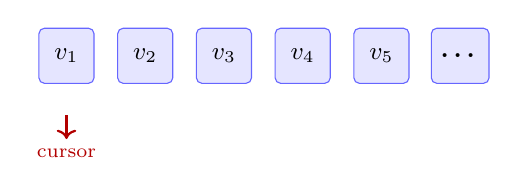
\begin{tikzpicture}
    \foreach \i/\lab in {0/$v_1$, 1/$v_2$, 2/$v_3$, 3/$v_4$, 4/$v_5$,
                         5/\dots} {
      \node[draw=blue!60, fill=blue!10, minimum size=7mm,
            rounded corners=2pt, font=\small\bfseries] (n\i)
        at (\i*1.0, 0) {\lab};
    }
    \draw[->, thick, red!70!black] ([yshift=-4mm]n0.south)
      -- ++(0,-3mm) node[below, font=\scriptsize] {cursor};
  \end{tikzpicture}

  \bigskip
  \raggedright
  \begin{description}[\texttt{lookahead}~~]
    \item[\texttt{extract(hdr)}]
      Pop first $n$ bits, bind to \texttt{hdr}.\\
      {\small If list exhausted $\;\to\;$
       \texttt{\textcolor{red!70!black}{PacketTooShort}}.}
    \item[\texttt{lookahead}]
      Peek at front without consuming.
    \item[\texttt{advance}]
      Consume and \emph{discard} (no binding).
  \end{description}
\end{frame}
% \end{column}

% \begin{column}{0.48\textwidth}
% \textbf{\centering Symbolic}\par\medskip
% \begin{block}{}
% Two lists: \textbf{input} (read from) + \textbf{construction} (built during parsing).

% \smallskip
% {\footnotesize\textcolor{gray}{Input forms:}}\\[2pt]
% \begin{tikzpicture}
%   \node[draw=orange!70, fill=orange!60, minimum size=5mm, rounded corners=1pt, font=\scriptsize\bfseries, text=white] at (0, 0) {$\infty$};
%   \node[font=\scriptsize, anchor=west] at (0.5, 0) {fully symbolic, arbitrary length};
% \end{tikzpicture}\\[2pt]
% \begin{tikzpicture}
%   \foreach \i/\lab in {0/$v_1$, 1/$v_2$, 2/\dots, 3/$v_k$} {
%     \node[draw=orange!60, fill=yellow!20, minimum size=5mm, rounded corners=1pt, font=\scriptsize\bfseries, text=yellow!30!black] at (\i*0.85, 0) {\lab};
%   }
%   \node[font=\scriptsize, anchor=west] at (3.6, 0) {known length};
% \end{tikzpicture}\\[2pt]
% \begin{tikzpicture}
%   \foreach \i/\lab in {0/$v_1$, 1/\dots, 2/$v_k$} {
%     \node[draw=orange!60, fill=yellow!20, minimum size=5mm, rounded corners=1pt, font=\scriptsize\bfseries, text=yellow!30!black] at (\i*0.85, 0) {\lab};
%   }
%   \node[draw=orange!70, fill=orange!60, minimum size=5mm, rounded corners=1pt, font=\scriptsize\bfseries, text=white] at (2.55, 0) {$\infty$};
%   \node[font=\scriptsize, anchor=west] at (3.1, 0) {prefix + tail};
% \end{tikzpicture}

% \medskip
% \textbf{extract:} if value $\to$ pop \& bind.\\
% If $\infty$ $\to$ fresh symbolic, bind \& add to construction list.

% \smallskip
% \textbf{lookahead:} peek; if $\infty$ $\to$ fresh symbolic appended to input.

% \smallskip
% \textbf{advance:} values $\to$ construction list;\\
% if $\infty$ $\to$ fresh symbolic to construction.

% \smallskip
% \textbf{Final packet} = construction list ++ remaining input.
% \end{block}
% \end{column}
% \end{columns}
% \end{frame}

% ============================================================
% SYMBOLIC PACKET MODEL
% ============================================================
\begin{frame}{Packet Model: Symbolic}

  In symbolic mode the packet may not be known a priori.\\[2pt]
  The interpreter maintains \textbf{two} lists:

\vspace{0.5cm}  % <--- Vertical space before the whole block
  \hspace*{1.5cm} % <--- Indent the whole thing from the left margin
  %
  \begin{tabular}{c}
    \textcolor{blue!70}{\textbf{Input list}}\\[2pt]
    {\small read from}
  \end{tabular}
  %
  \hspace{0.5cm} % <--- Space between Left and +
  {\Large +}
  \hspace{0.5cm} % <--- Space between + and Right
  %
  \begin{tabular}{c}
    \textcolor{orange!80!black}{\textbf{Construction list}}\\[2pt]
    {\small built during parsing}
  \end{tabular}
  \bigskip

  The input list takes one of three forms:

  \medskip
  \centering
  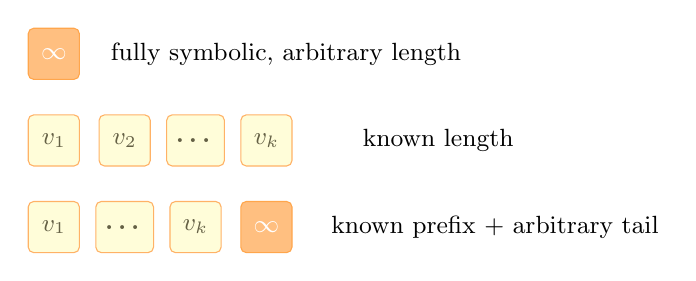
\begin{tikzpicture}[
      cell/.style={draw=orange!60, fill=yellow!15, minimum size=6.5mm,
                   rounded corners=2pt, font=\small\bfseries,
                   text=yellow!30!black},
      inf/.style={draw=orange!70, fill=orange!50, minimum size=6.5mm,
                  rounded corners=2pt, font=\small\bfseries, text=white},
      lbl/.style={font=\small, anchor=west}
    ]
    % Row 1: fully symbolic
    \node[inf] at (0, 0) {$\infty$};
    \node[lbl] at (0.6, 0) {fully symbolic, arbitrary length};

    % Row 2: known length
    \foreach \i/\lab in {0/$v_1$, 1/$v_2$, 2/\dots, 3/$v_k$}
      \node[cell] at (\i*0.9, -1.1) {\lab};
    \node[lbl] at (3.8, -1.1) {known length};

    % Row 3: prefix + tail
    \foreach \i/\lab in {0/$v_1$, 1/\dots, 2/$v_k$}
      \node[cell] at (\i*0.9, -2.2) {\lab};
    \node[inf] at (2.7, -2.2) {$\infty$};
    \node[lbl] at (3.4, -2.2) {known prefix + arbitrary tail};
  \end{tikzpicture}

  \medskip
  \raggedright
  {\small Each $v_i$ may itself be concrete \emph{or} symbolic.}
\end{frame}

% \begin{frame}{Packet Model: Symbolic}
% Two lists: \textbf{input} (read from) + \textbf{construction} (built during parsing).

% \textbf{lookahead:} peek; if $\infty$ $\to$ fresh symbolic appended to input.

% \pause

% the input packet is given by  concatenating the construction list with what remains in the input lis

% the output packet is given by ...

% \end{frame}

\begin{frame}{Packet Model: Symbolic — Operations}

  \begin{description}[\texttt{lookahead}~~]
    \item[\texttt{extract(hdr)}]
      \begin{itemize}
        \item Input empty $\;\to\;$
              \texttt{\textcolor{red!70!black}{PacketTooShort}}.
        \item Head is a value $\;\to\;$ pop, bind to \texttt{hdr},
              append to construction list.
        \item Head is $\infty$ $\;\to\;$ generate \emph{fresh symbolic}
              value, bind \& append to construction list.
      \end{itemize}

    \medskip
    \item[\texttt{lookahead}]
      Peek without advancing the cursor.
      \begin{itemize}
        \item Head is a value $\;\to\;$ return it.
        \item Head is $\infty$ $\;\to\;$ generate fresh symbolic,
              \textbf{prepend to input list} (not bound).
      \end{itemize}

    \medskip
    \item[\texttt{advance}]
      Consume without binding.
      \begin{itemize}
        \item Values $\;\to\;$ move from input to construction list.
        \item $\infty$ $\;\to\;$ fresh symbolic added directly to
              construction list.
      \end{itemize}
  The final output packet consists of the deparsed header + any remaining input (the packet payload)
  \end{description}
\end{frame}

\begin{frame}{Why the Construction List? \quad (1) Counterexamples}

  Consider a fully symbolic input $[\infty]$:

  \medskip
  \begin{enumerate}
    \item \texttt{extract} 2 bits $\;\to\;$ fresh symbolic $a$
    \item \texttt{advance} 2 bits $\;\to\;$ fresh symbolic $b$
          {\small\textcolor{gray}{(not bound)}}
    \item \texttt{extract} 2 bits $\;\to\;$ fresh symbolic $c$
  \end{enumerate}

  \bigskip
  \centering
  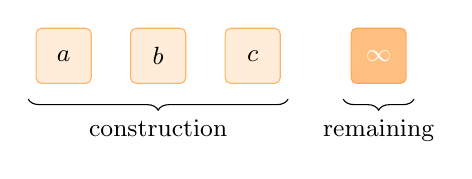
\begin{tikzpicture}[
      cell/.style={draw=orange!60, fill=orange!15, minimum size=7mm,
                   rounded corners=2pt, font=\small\bfseries},
      inf/.style={draw=orange!70, fill=orange!50, minimum size=7mm,
                  rounded corners=2pt, font=\small\bfseries, text=white},
      >=stealth
    ]
    \node[cell] at (0,0) {$a$};
    \node[cell] at (1.2,0) {$b$};
    \node[cell] at (2.4,0) {$c$};
    \node[inf]  at (4.0,0) {$\infty$};
    \draw[decorate, decoration={brace, mirror, amplitude=4pt}]
      (-0.45,-0.55) -- (2.85,-0.55)
      node[midway, below=4pt, font=\small] {construction};
    \draw[decorate, decoration={brace, mirror, amplitude=4pt}]
      (3.55,-0.55) -- (4.45,-0.55)
      node[midway, below=4pt, font=\small] {remaining};
  \end{tikzpicture}

  \bigskip
  \raggedright
  Suppose the deparser emits $a \mathbin{\|} c$. Then the full output packet is $ a \mathbin{\|} c \mathbin{\|}  \infty$
  {\small\textcolor{gray}{(payload unaffected)}}.

  \smallskip
  When a counterexample is found, the solver assigns a concrete value to
  each symbolic variable ($a$, $b$, $c$). The construction list
  \textbf{preserves their original order} in the packet.
  % We could maybe use something like the variable id to encode this cheaper ?? 
\end{frame}

% ============================================================
% WHY THE CONSTRUCTION LIST? — LOOKAHEAD
% ============================================================
\begin{frame}{Why the Construction List? \quad (2) Lookahead}

  Consider a fully symbolic input $[\infty]$:

  \medskip
  \begin{enumerate}
    \item \texttt{extract} 2 bits $\;\to\;$ fresh symbolic $a$
    \item \texttt{lookahead} 2 bits $\;\to\;$ fresh symbolic $b$
          {\small\textcolor{gray}{(peeked, not consumed)}}
  \end{enumerate}

  \bigskip
  \centering
  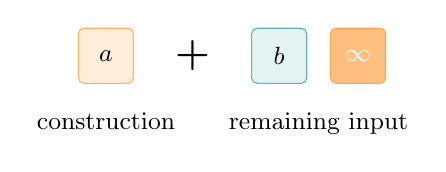
\begin{tikzpicture}[
      cell/.style={draw=orange!60, fill=orange!15, minimum size=7mm,
                   rounded corners=2pt, font=\small\bfseries},
      cellg/.style={draw=teal!60, fill=teal!10, minimum size=7mm,
                    rounded corners=2pt, font=\small\bfseries},
      inf/.style={draw=orange!70, fill=orange!50, minimum size=7mm,
                  rounded corners=2pt, font=\small\bfseries, text=white},
    ]
    % construction
    \node[cell] at (0,0) {$a$};
    \node[font=\small, below=2mm] at (0,-0.4) {construction};

    \node[font=\Large\bfseries] at (1.1,0) {+};

    % remaining input
    \node[cellg] at (2.2,0) {$b$};
    \node[inf]   at (3.2,0) {$\infty$};
    \node[font=\small, below=2mm] at (2.7,-0.4) {remaining input};
  \end{tikzpicture}

  \bigskip
  \raggedright
  The deparser emits only $a$, but $b$ stays in the remaining input
  (part of the payload).

  \smallskip
  \textbf{Something about composing two programs }
  This is very much an edge case
\end{frame}

\begin{frame}{Table}
\end{frame}

\begin{frame}{parser cycles}
\end{frame}

% \begin{frame}
% Why do we need the construction list? to generate counterexample input packets 

% consider we have an inf input packet

% we extract 2 bits (a) from it, len we advance two bits b and extract two bits c from it again. 
% lets say we deparse these in the same order, so the output packet is a + c + infty (infty is the payload which is unaffected by tge )
% now if we come up with a counterexample in this branch. a counterexample must be atleat length 6 
% \end{frame}

% \begin{frame}
% Why do we need the construction list? To model lookahead 

% Another example 

% consider we have a inf input packet, we extract 2 bits a , then lookahead 2 more bits b
% we output a from the deparser, but 
% \end{frame}

% \begin{frame} {Parser Model}
% \end{frame}

% \begin{frame}{Network Model}
% \centering
% \begin{tikzpicture}[
%   x=1cm, y=1cm,
%   switch/.style={rectangle, draw=blue!50!black, fill=blue!5,
%                  rounded corners=4pt, minimum width=1.6cm, minimum height=1.2cm,
%                  align=center, font=\small\sffamily},
%   host/.style={rectangle, draw=green!50!black, fill=green!8,
%                rounded corners=4pt, minimum width=1.4cm, minimum height=0.9cm,
%                align=center, font=\small\sffamily},
%   queue/.style={rectangle, draw=orange!70!black, fill=orange!10,
%                 rounded corners=2pt, minimum width=1.0cm, minimum height=0.4cm,
%                 font=\scriptsize\sffamily, align=center},
%   link/.style={-{Stealth[length=3pt]}, thick, blue!60!black},
%   lbl/.style={font=\sffamily\fontsize{6}{7}\selectfont, text=gray!70},
% ]

% %% ===== HOSTS (generators) =====
% \node[host] (h1) at (-4.8, 1.2) {\textbf{Host} $H_1$\\[-1pt]\scriptsize generator};
% \node[host] (h2) at (-4.8,-1.2) {\textbf{Host} $H_2$\\[-1pt]\scriptsize generator};

% %% ===== INGRESS QUEUES =====
% \node[queue] (q1) at (-2.7, 1.2) {$\langle p_1, p_2, \dots\rangle$};
% \node[queue] (q2) at (-2.7,-1.2) {$\langle p_3, p_4, \dots\rangle$};

% %% ===== SWITCHES =====
% \node[switch] (s1) at (-0.3, 1.2) {\textbf{Switch} $s_1$\\[-1pt]\scriptsize P4 program};
% \node[switch] (s2) at (-0.3,-1.2) {\textbf{Switch} $s_2$\\[-1pt]\scriptsize P4 program};
% \node[switch] (s3) at (3.2, 0)   {\textbf{Switch} $s_3$\\[-1pt]\scriptsize P4 program};

% %% ===== INTER-SWITCH QUEUES =====
% \node[queue] (q12) at (-0.3, 0)   {\scriptsize queue};
% \node[queue] (q13) at (1.7, 0.9)  {\scriptsize queue};
% \node[queue] (q23) at (1.7,-0.9)  {\scriptsize queue};

% %% ===== OUTPUT HOST =====
% \node[host, fill=red!8, draw=red!40!black] (sink) at (6.2, 0)
%   {\textbf{Host} $H_3$\\[-1pt]\scriptsize sink};
% \node[queue] (q3out) at (5.0, 0) {$\langle \dots \rangle$};

% %% ===== EDGES =====
% \draw[link] (h1) -- (q1);
% \draw[link] (h2) -- (q2);
% \draw[link] (q1) -- (s1);
% \draw[link] (q2) -- (s2);

% \draw[link] (s1) -- (q12);  \draw[link] (q12) -- (s2);
% \draw[link] (s1) -- (q13);  \draw[link] (q13) -- (s3);
% \draw[link] (s2) -- (q23);  \draw[link] (q23) -- (s3);

% \draw[link] (s3) -- (q3out);
% \draw[link] (q3out) -- (sink);

% %% ===== LOCKSTEP BOX =====
% \begin{scope}[on background layer]
%   \node[draw=red!40!black, dashed, thick, rounded corners=8pt, fill=red!3,
%         inner sep=10pt,
%         fit=(s1)(s2)(s3)(q12)(q13)(q23),
%         label={[font=\sffamily\scriptsize\bfseries, text=red!50!black]above:lockstep --- one tick per step}] {};
% \end{scope}

% \end{tikzpicture}

% \medskip
% \begin{columns}[T]
% \begin{column}{0.48\textwidth}
% \small
% \textbf{Simulation loop (per tick):}
% \begin{enumerate}\setlength\itemsep{2pt}
%   \item Hosts \textbf{generate} packets into ingress queues
%   \item Every switch \textbf{dequeues} the head packet
%   \item P4 program executes $\to$ 0, 1, or $n$ output packets
%   \item Outputs \textbf{enqueued} on the destination link
% \end{enumerate}
% \end{column}
% \begin{column}{0.48\textwidth}
% \small
% \textbf{Design choices:}
% \begin{itemize}\setlength\itemsep{2pt}
%   \item All switches execute \textbf{synchronously} (lockstep)
%   \item Link queues model \textbf{in-flight} packets
%   \item Clone / multicast: one input $\to$ multiple outputs
%   \item Register state persists \textbf{within} each switch across ticks
% \end{itemize}
% \end{column}
% \end{columns}
% \end{frame}

\begin{frame}{Network Model}
\footfullcite{10.1145/2676726.2676990}
       \small
       Inspired by the approach from Bjørner et al. (POPL 2015), a network
      $\mathcal{N}$ consists of:
       
       \begin{itemize}
         \item \textbf{Nodes ($N$):} A finite set of devices.
         \item \textbf{Ports ($Ports(n)$):} The set of ports for each node $n
      \in N$.
         \item \textbf{Connections ($\gamma$):} A link relation on
      $Port_\mathcal{N} = \{n.p \mid n \in N, p \in Ports(n)\}$ that is:
         \begin{itemize}
          \item \textbf{Symmetric:} $n.p \ \gamma \ n'.p' \implies n'.p' \
      \gamma \ n.p$
          \item \textbf{Irreflexive:} $\neg(n.p \ \gamma \ n.p)$ (no
      self-loops)
          \item \textbf{1-to-1:} Each port connects to at most one other port.
        \end{itemize}
      \end{itemize}
   
      \pause
      \begin{block}{Network State $\Sigma = (\mathcal{S}, \mathcal{Q})$}
        \begin{enumerate}
          \item \textbf{Global State ($\mathcal{S}$):} A mapping $\mathcal{S}
      : N \to S$ from nodes to their local pipeline states.
      %     Transitions are modeled as: $\langle s, \pi, p \rangle \rightarrow
      % \langle s', [(p_i, \pi_i)]_{i=1}^n \rangle$
          \item \textbf{In-flight Packets ($\mathcal{Q}$):} A mapping from
      each port to a \textbf{sequence} of packets:
         $ \mathcal{Q} : Port_\mathcal{N} \to
      (\text{Packet})^* $
          \begin{itemize}
            \item Chronological FIFO ordering between time steps, with non-deterministic ordering of
      packets arriving simultaneously at the same step.
          \end{itemize}
        \end{enumerate}
      \end{block}
\end{frame}

\begin{frame}{Network Model --- Concrete Example}
\centering
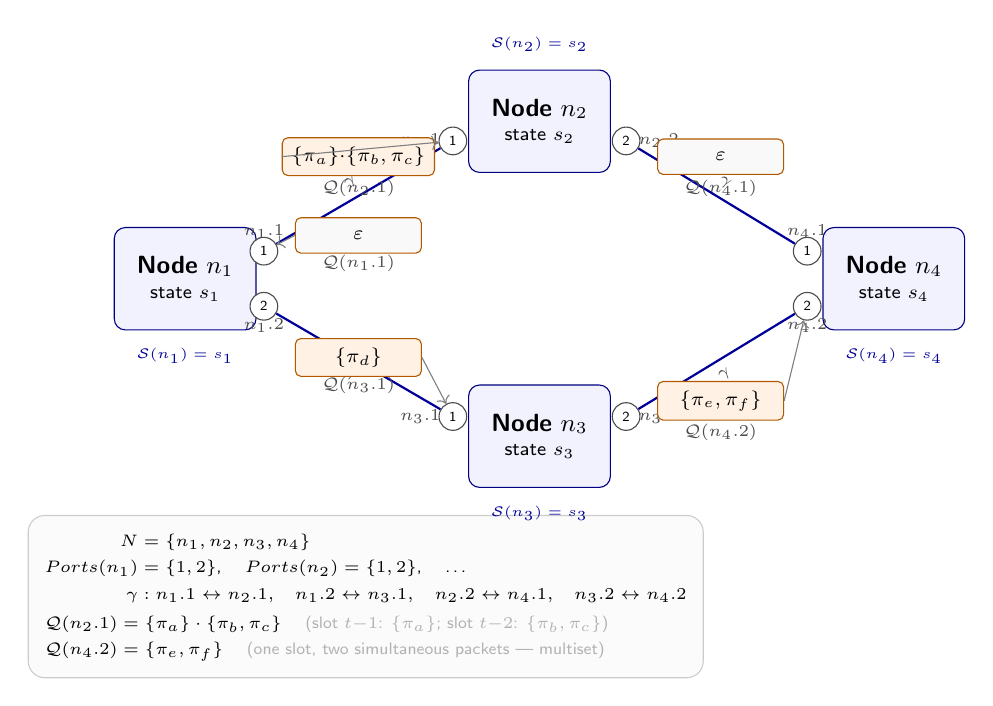
\begin{tikzpicture}[
  x=1cm, y=1cm,
  node box/.style={rectangle, draw=blue!50!black, fill=blue!5,
                   rounded corners=4pt, minimum width=1.8cm, minimum height=1.3cm,
                   align=center, font=\small\sffamily},
  port/.style={circle, draw=black!70, fill=white,
               inner sep=0pt, minimum size=10pt,
               font=\sffamily\fontsize{5}{6}\selectfont},
  queuebox/.style={rectangle, draw=orange!70!black, fill=orange!10,
                   rounded corners=2pt, minimum width=1.6cm, minimum height=0.45cm,
                   font=\scriptsize\sffamily, align=center},
  conn/.style={thick, blue!60!black},
  pktA/.style={rectangle, draw=violet!70!black, fill=violet!15,
               rounded corners=1pt, minimum width=0.35cm, minimum height=0.25cm,
               font=\sffamily\fontsize{4}{5}\selectfont, inner sep=1pt},
  pktB/.style={rectangle, draw=teal!70!black, fill=teal!15,
               rounded corners=1pt, minimum width=0.35cm, minimum height=0.25cm,
               font=\sffamily\fontsize{4}{5}\selectfont, inner sep=1pt},
  lbl/.style={font=\sffamily\fontsize{6}{7}\selectfont, text=gray!60!black},
  statelbl/.style={font=\sffamily\fontsize{5.5}{6.5}\selectfont, text=blue!60!black},
]

%% ===== NODES =====
\node[node box] (n1) at (-3.5, 0) {\textbf{Node} $n_1$\\[-2pt]\scriptsize state $s_1$};
\node[node box] (n2) at ( 1.0, 2.0) {\textbf{Node} $n_2$\\[-2pt]\scriptsize state $s_2$};
\node[node box] (n3) at ( 1.0,-2.0) {\textbf{Node} $n_3$\\[-2pt]\scriptsize state $s_3$};
\node[node box] (n4) at ( 5.5, 0) {\textbf{Node} $n_4$\\[-2pt]\scriptsize state $s_4$};

%% ===== PORTS (small circles on node borders) =====
% n1 ports
\node[port] (n1p1) at (-2.5, 0.35) {\tiny 1};
\node[port] (n1p2) at (-2.5,-0.35) {\tiny 2};

% n2 ports
\node[port] (n2p1) at (-0.1, 1.75) {\tiny 1};
\node[port] (n2p2) at ( 2.1, 1.75) {\tiny 2};

% n3 ports
\node[port] (n3p1) at (-0.1,-1.75) {\tiny 1};
\node[port] (n3p2) at ( 2.1,-1.75) {\tiny 2};

% n4 ports
\node[port] (n4p1) at (4.4, 0.35) {\tiny 1};
\node[port] (n4p2) at (4.4,-0.35) {\tiny 2};

%% ===== PORT LABELS =====
\node[lbl, above=1pt] at (n1p1) {$n_1.1$};
\node[lbl, below=1pt] at (n1p2) {$n_1.2$};
\node[lbl, left=1pt]  at (n2p1) {$n_2.1$};
\node[lbl, right=1pt] at (n2p2) {$n_2.2$};
\node[lbl, left=1pt]  at (n3p1) {$n_3.1$};
\node[lbl, right=1pt] at (n3p2) {$n_3.2$};
\node[lbl, above=1pt] at (n4p1) {$n_4.1$};
\node[lbl, below=1pt] at (n4p2) {$n_4.2$};

%% ===== CONNECTIONS (gamma) =====
\draw[conn] (n1p1) -- (n2p1)
  node[midway, above, sloped, lbl] {$\gamma$};
\draw[conn] (n1p2) -- (n3p1)
  node[midway, below, sloped, lbl] {$\gamma$};
\draw[conn] (n2p2) -- (n4p1)
  node[midway, above, sloped, lbl] {$\gamma$};
\draw[conn] (n3p2) -- (n4p2)
  node[midway, below, sloped, lbl] {$\gamma$};

%% ===== IN-FLIGHT QUEUES (shown as packet sequences near ports) =====

% Queue on link n1.1 -> n2.1: two timestep slots
\node[queuebox] (qA) at (-1.3, 1.55) {$\{\pi_a\}{\cdot}\{\pi_b,\pi_c\}$};
\draw[->, thin, gray] (qA.west) -- (n2p1);
\node[lbl] at (-1.3, 1.15) {$\mathcal{Q}(n_2.1)$};

% Queue on link n2.1 -> n1.1: empty
\node[queuebox, fill=gray!5] (qAr) at (-1.3, 0.55) {$\varepsilon$};
\draw[->, thin, gray] (qAr.west) -- (n1p1);
\node[lbl] at (-1.3, 0.2) {$\mathcal{Q}(n_1.1)$};

% Queue on link n1.2 -> n3.1
\node[queuebox] (qB) at (-1.3,-1.0) {$\{\pi_d\}$};
\draw[->, thin, gray] (qB.east) -- (n3p1);
\node[lbl] at (-1.3,-1.35) {$\mathcal{Q}(n_3.1)$};

% Queue on link n2.2 -> n4.1
\node[queuebox, fill=gray!5] (qC) at (3.3, 1.55) {$\varepsilon$};
\node[lbl] at (3.3, 1.15) {$\mathcal{Q}(n_4.1)$};

% Queue on link n3.2 -> n4.2
\node[queuebox] (qD) at (3.3,-1.55) {$\{\pi_e, \pi_f\}$};
\draw[->, thin, gray] (qD.east) -- (n4p2);
\node[lbl] at (3.3,-1.95) {$\mathcal{Q}(n_4.2)$};

%% ===== STATE ANNOTATION =====
\node[statelbl, below=3pt] at (n1.south) {$\mathcal{S}(n_1) = s_1$};
\node[statelbl, above=3pt] at (n2.north) {$\mathcal{S}(n_2) = s_2$};
\node[statelbl, below=3pt] at (n3.south) {$\mathcal{S}(n_3) = s_3$};
\node[statelbl, below=3pt] at (n4.south) {$\mathcal{S}(n_4) = s_4$};

%% ===== LEGEND BOX =====
\begin{scope}[on background layer]
  \node[draw=gray!40, rounded corners=6pt, fill=gray!3,
        inner sep=6pt, anchor=north west,
        font=\sffamily\fontsize{6}{7.5}\selectfont]
    at (-5.5, -3.0) {%
    \begin{tabular}{@{}r@{\ }l@{}}
      $N$ &$= \{n_1, n_2, n_3, n_4\}$ \\[2pt]
      $Ports(n_1)$ &$= \{1,2\}$, \quad $Ports(n_2) = \{1,2\}$, \quad \ldots \\[2pt]
      $\gamma$ &$: n_1.1 \leftrightarrow n_2.1, \quad
                    n_1.2 \leftrightarrow n_3.1, \quad
                    n_2.2 \leftrightarrow n_4.1, \quad
                    n_3.2 \leftrightarrow n_4.2$ \\[3pt]
      \multicolumn{2}{@{}l}{$\mathcal{Q}(n_2.1) = \{\pi_a\} \cdot \{\pi_b, \pi_c\}$
        \quad {\color{gray!60}(slot $t{-}1$: $\{\pi_a\}$; slot $t{-}2$: $\{\pi_b,\pi_c\}$)}} \\[2pt]
      \multicolumn{2}{@{}l}{$\mathcal{Q}(n_4.2) = \{\pi_e, \pi_f\}$
        \quad {\color{gray!60}(one slot, two simultaneous packets --- multiset)}}
    \end{tabular}
  };
\end{scope}

\end{tikzpicture}
\end{frame}

\begin{frame}{Network Model --- Topology Example}
\centering
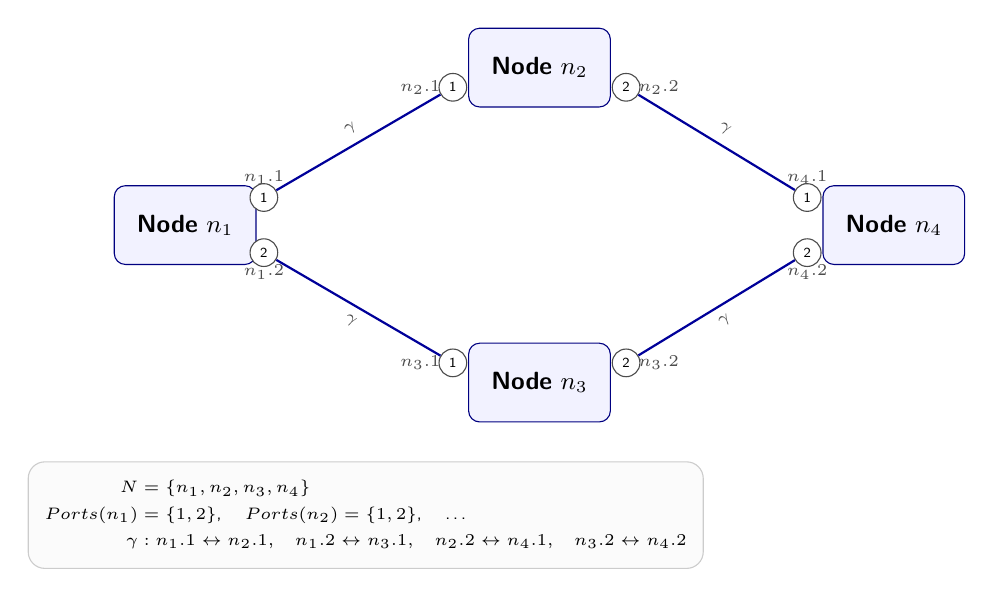
\begin{tikzpicture}[
  x=1cm, y=1cm,
  node box/.style={rectangle, draw=blue!50!black, fill=blue!5,
                   rounded corners=4pt, minimum width=1.8cm, minimum height=1.0cm,
                   align=center, font=\small\sffamily},
  port/.style={circle, draw=black!70, fill=white,
               inner sep=0pt, minimum size=10pt,
               font=\sffamily\fontsize{5}{6}\selectfont},
  conn/.style={thick, blue!60!black},
  lbl/.style={font=\sffamily\fontsize{6}{7}\selectfont, text=gray!60!black}
]

%% ===== NODES =====
\node[node box] (n1) at (-3.5, 0) {\textbf{Node} $n_1$};
\node[node box] (n2) at ( 1.0, 2.0) {\textbf{Node} $n_2$};
\node[node box] (n3) at ( 1.0,-2.0) {\textbf{Node} $n_3$};
\node[node box] (n4) at ( 5.5, 0) {\textbf{Node} $n_4$};

%% ===== PORTS (small circles on node borders) =====
% n1 ports
\node[port] (n1p1) at (-2.5, 0.35) {\tiny 1};
\node[port] (n1p2) at (-2.5,-0.35) {\tiny 2};

% n2 ports
\node[port] (n2p1) at (-0.1, 1.75) {\tiny 1};
\node[port] (n2p2) at ( 2.1, 1.75) {\tiny 2};

% n3 ports
\node[port] (n3p1) at (-0.1,-1.75) {\tiny 1};
\node[port] (n3p2) at ( 2.1,-1.75) {\tiny 2};

% n4 ports
\node[port] (n4p1) at (4.4, 0.35) {\tiny 1};
\node[port] (n4p2) at (4.4,-0.35) {\tiny 2};

%% ===== PORT LABELS =====
\node[lbl, above=1pt] at (n1p1) {$n_1.1$};
\node[lbl, below=1pt] at (n1p2) {$n_1.2$};
\node[lbl, left=1pt]  at (n2p1) {$n_2.1$};
\node[lbl, right=1pt] at (n2p2) {$n_2.2$};
\node[lbl, left=1pt]  at (n3p1) {$n_3.1$};
\node[lbl, right=1pt] at (n3p2) {$n_3.2$};
\node[lbl, above=1pt] at (n4p1) {$n_4.1$};
\node[lbl, below=1pt] at (n4p2) {$n_4.2$};

%% ===== CONNECTIONS (gamma) =====
\draw[conn] (n1p1) -- (n2p1)
  node[midway, above, sloped, lbl] {$\gamma$};
\draw[conn] (n1p2) -- (n3p1)
  node[midway, below, sloped, lbl] {$\gamma$};
\draw[conn] (n2p2) -- (n4p1)
  node[midway, above, sloped, lbl] {$\gamma$};
\draw[conn] (n3p2) -- (n4p2)
  node[midway, below, sloped, lbl] {$\gamma$};

%% ===== LEGEND BOX =====
\begin{scope}[on background layer]
  \node[draw=gray!40, rounded corners=6pt, fill=gray!3,
        inner sep=6pt, anchor=north west,
        font=\sffamily\fontsize{6}{7.5}\selectfont]
    at (-5.5, -3.0) {%
    \begin{tabular}{@{}r@{\ }l@{}}
      $N$ &$= \{n_1, n_2, n_3, n_4\}$ \\[2pt]
      $Ports(n_1)$ &$= \{1,2\}$, \quad $Ports(n_2) = \{1,2\}$, \quad \ldots \\[2pt]
      $\gamma$ &$: n_1.1 \leftrightarrow n_2.1, \quad
                    n_1.2 \leftrightarrow n_3.1, \quad
                    n_2.2 \leftrightarrow n_4.1, \quad
                    n_3.2 \leftrightarrow n_4.2$
    \end{tabular}
  };
\end{scope}

\end{tikzpicture}
\end{frame}

\begin{frame}{Network Model: Example}
\centering
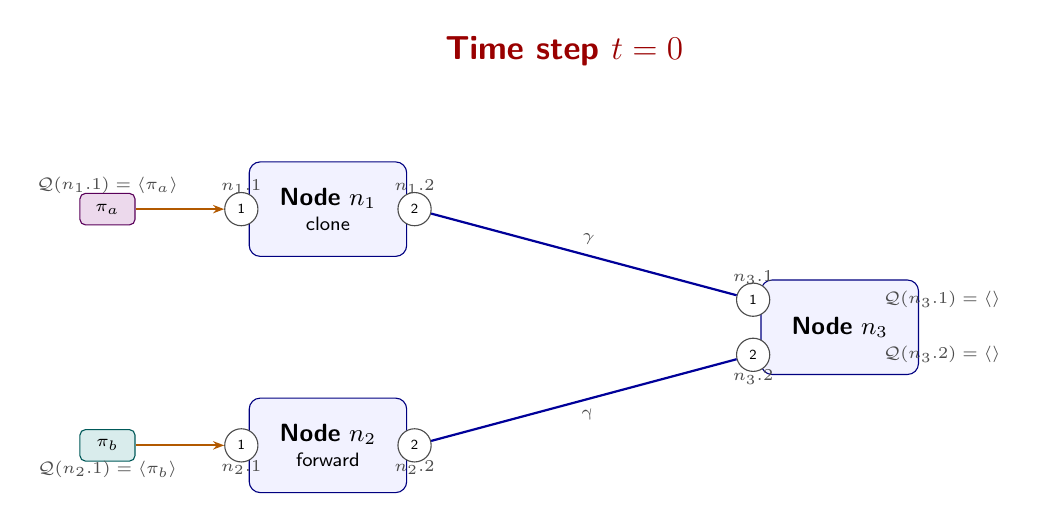
\begin{tikzpicture}[
  x=1cm, y=1cm,
  node box/.style={rectangle, draw=blue!50!black, fill=blue!5,
                   rounded corners=4pt, minimum width=2.0cm, minimum height=1.2cm,
                   align=center, font=\small\sffamily},
  port/.style={circle, draw=black!70, fill=white,
               inner sep=0pt, minimum size=12pt,
               font=\sffamily\fontsize{5}{6}\selectfont},
  conn/.style={thick, blue!60!black},
  pkt/.style={rectangle, draw=violet!70!black, fill=violet!15,
              rounded corners=2pt, minimum width=0.7cm, minimum height=0.4cm,
              font=\sffamily\fontsize{6}{7}\selectfont, inner sep=2pt},
  pktB/.style={rectangle, draw=teal!70!black, fill=teal!15,
              rounded corners=2pt, minimum width=0.7cm, minimum height=0.4cm,
              font=\sffamily\fontsize{6}{7}\selectfont, inner sep=2pt},
  lbl/.style={font=\sffamily\fontsize{6}{7}\selectfont, text=gray!60!black},
  steplbl/.style={font=\sffamily\bfseries\large, text=red!60!black},
  arrow/.style={-{Stealth[length=4pt]}, thick, orange!70!black},
]

%% ===== TIME LABEL =====
\node[steplbl] at (0, 3.5) {Time step $t = 0$};

%% ===== NODES =====
\node[node box] (n1) at (-3.0, 1.5) {\textbf{Node} $n_1$\\[-2pt]\scriptsize clone};
\node[node box] (n2) at (-3.0,-1.5) {\textbf{Node} $n_2$\\[-2pt]\scriptsize forward};
\node[node box] (n3) at ( 3.5, 0.0) {\textbf{Node} $n_3$};

%% ===== PORTS =====
% n1: port 1 (ingress, left), port 2 (egress to n3, right)
\node[port] (n1p1) at (-4.1, 1.5) {\tiny 1};
\node[port] (n1p2) at (-1.9, 1.5) {\tiny 2};

% n2: port 1 (ingress, left), port 2 (egress to n3, right)
\node[port] (n2p1) at (-4.1,-1.5) {\tiny 1};
\node[port] (n2p2) at (-1.9,-1.5) {\tiny 2};

% n3: port 1 (from n1, top-left), port 2 (from n2, bottom-left)
\node[port] (n3p1) at ( 2.4, 0.35) {\tiny 1};
\node[port] (n3p2) at ( 2.4,-0.35) {\tiny 2};

%% ===== PORT LABELS =====
\node[lbl, above=2pt] at (n1p1) {$n_1.1$};
\node[lbl, above=2pt] at (n1p2) {$n_1.2$};
\node[lbl, below=2pt] at (n2p1) {$n_2.1$};
\node[lbl, below=2pt] at (n2p2) {$n_2.2$};
\node[lbl, above=2pt] at (n3p1) {$n_3.1$};
\node[lbl, below=2pt] at (n3p2) {$n_3.2$};

%% ===== CONNECTIONS (gamma) =====
\draw[conn] (n1p2) -- (n3p1)
  node[midway, above, sloped, lbl] {$\gamma$};
\draw[conn] (n2p2) -- (n3p2)
  node[midway, below, sloped, lbl] {$\gamma$};

%% ===== INCOMING PACKETS AT t=0 =====
% Packet arriving at n1 ingress port
\node[pkt] (pktA) at (-5.8, 1.5) {$\pi_a$};
\draw[arrow] (pktA) -- (n1p1);
\node[lbl, above=2pt] at (pktA) {$\mathcal{Q}(n_1.1) = \langle \pi_a \rangle$};

% Packet arriving at n2 ingress port
\node[pktB] (pktB) at (-5.8,-1.5) {$\pi_b$};
\draw[arrow] (pktB) -- (n2p1);
\node[lbl, below=2pt] at (pktB) {$\mathcal{Q}(n_2.1) = \langle \pi_b \rangle$};

%% ===== EMPTY QUEUES on n3 side =====
\node[lbl] at (4.8, 0.35) {$\mathcal{Q}(n_3.1) = \langle\rangle$};
\node[lbl] at (4.8,-0.35) {$\mathcal{Q}(n_3.2) = \langle\rangle$};

%% ===== ANNOTATION: what will happen =====
% \node[draw=blue!30, fill=blue!3, rounded corners=4pt, 
%       font=\sffamily\fontsize{6.5}{8}\selectfont, align=left,
%       anchor=north west, text width=5.5cm]
%   at (-5.8, -2.8) {%
%   \textbf{Pending transitions:}\\[3pt]
%   $n_1$: $\langle s_1,\, \pi_a,\, 1 \rangle 
%          \to \langle s_1',\, [(2,\, \pi_a'),\, (2,\, \pi_a'')]  \rangle$\\
%   \quad\scriptsize(clone: one input $\to$ two outputs on port 2)\\[3pt]
%   $n_2$: $\langle s_2,\, \pi_b,\, 1 \rangle 
%          \to \langle s_2',\, [(2,\, \pi_b')]  \rangle$\\
%   \quad\scriptsize(forward: one input $\to$ one output on port 2)
%   };

%% ===== LEGEND =====
% \node[draw=gray!40, rounded corners=4pt, fill=gray!3,
%       inner sep=5pt, anchor=north west,
%       font=\sffamily\fontsize{6}{7.5}\selectfont]
%   at (1.5, -2.8) {%
%   \begin{tabular}{@{}r@{\ }l@{}}
%     $N$ &$= \{n_1, n_2, n_3\}$ \\[2pt]
%     $\gamma$ &$: n_1.2 \leftrightarrow n_3.1$\\
%              &$\phantom{:}\ n_2.2 \leftrightarrow n_3.2$
%   \end{tabular}
%   };

\end{tikzpicture}
\end{frame}


\begin{frame}{Network Model:}
\centering
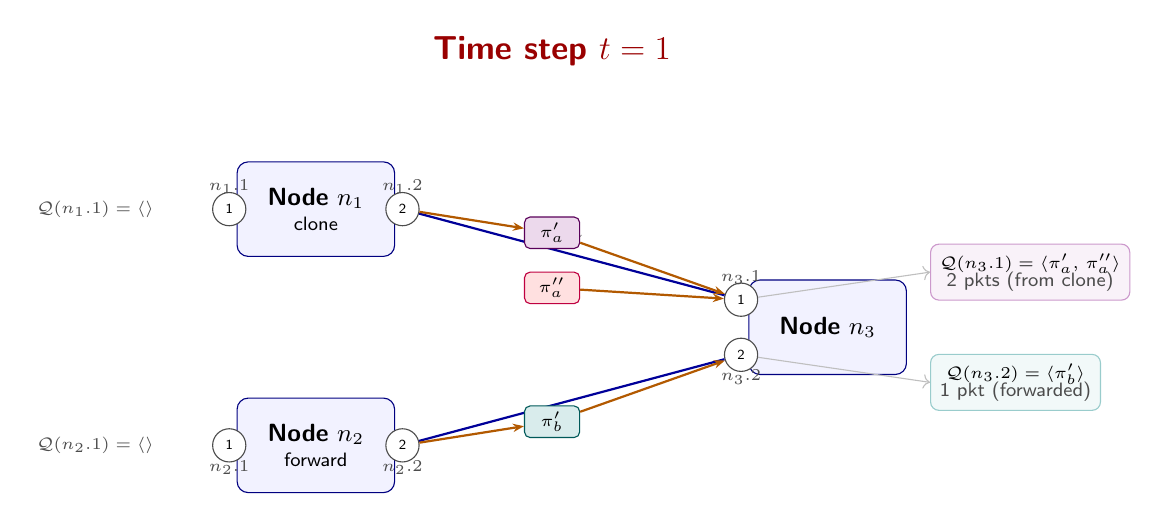
\begin{tikzpicture}[
  x=1cm, y=1cm,
  node box/.style={rectangle, draw=blue!50!black, fill=blue!5,
                   rounded corners=4pt, minimum width=2.0cm, minimum height=1.2cm,
                   align=center, font=\small\sffamily},
  port/.style={circle, draw=black!70, fill=white,
               inner sep=0pt, minimum size=12pt,
               font=\sffamily\fontsize{5}{6}\selectfont},
  conn/.style={thick, blue!60!black},
  pkt/.style={rectangle, draw=violet!70!black, fill=violet!15,
              rounded corners=2pt, minimum width=0.7cm, minimum height=0.4cm,
              font=\sffamily\fontsize{6}{7}\selectfont, inner sep=2pt},
  pktC/.style={rectangle, draw=violet!50!red, fill=red!12,
              rounded corners=2pt, minimum width=0.7cm, minimum height=0.4cm,
              font=\sffamily\fontsize{6}{7}\selectfont, inner sep=2pt},
  pktB/.style={rectangle, draw=teal!70!black, fill=teal!15,
              rounded corners=2pt, minimum width=0.7cm, minimum height=0.4cm,
              font=\sffamily\fontsize{6}{7}\selectfont, inner sep=2pt},
  lbl/.style={font=\sffamily\fontsize{6}{7}\selectfont, text=gray!60!black},
  steplbl/.style={font=\sffamily\bfseries\large, text=red!60!black},
  arrow/.style={-{Stealth[length=4pt]}, thick, orange!70!black},
  donearrow/.style={-{Stealth[length=4pt]}, thick, green!50!black},
]

%% ===== TIME LABEL =====
\node[steplbl] at (0, 3.5) {Time step $t = 1$};

%% ===== NODES =====
\node[node box] (n1) at (-3.0, 1.5) {\textbf{Node} $n_1$\\[-2pt]\scriptsize clone};
\node[node box] (n2) at (-3.0,-1.5) {\textbf{Node} $n_2$\\[-2pt]\scriptsize forward};
\node[node box] (n3) at ( 3.5, 0.0) {\textbf{Node} $n_3$};

%% ===== PORTS =====
\node[port] (n1p1) at (-4.1, 1.5) {\tiny 1};
\node[port] (n1p2) at (-1.9, 1.5) {\tiny 2};

\node[port] (n2p1) at (-4.1,-1.5) {\tiny 1};
\node[port] (n2p2) at (-1.9,-1.5) {\tiny 2};

\node[port] (n3p1) at ( 2.4, 0.35) {\tiny 1};
\node[port] (n3p2) at ( 2.4,-0.35) {\tiny 2};

%% ===== PORT LABELS =====
\node[lbl, above=2pt] at (n1p1) {$n_1.1$};
\node[lbl, above=2pt] at (n1p2) {$n_1.2$};
\node[lbl, below=2pt] at (n2p1) {$n_2.1$};
\node[lbl, below=2pt] at (n2p2) {$n_2.2$};
\node[lbl, above=2pt] at (n3p1) {$n_3.1$};
\node[lbl, below=2pt] at (n3p2) {$n_3.2$};

%% ===== CONNECTIONS (gamma) =====
\draw[conn] (n1p2) -- (n3p1)
  node[midway, above, sloped, lbl] {$\gamma$};
\draw[conn] (n2p2) -- (n3p2)
  node[midway, below, sloped, lbl] {$\gamma$};

%% ===== INGRESS QUEUES NOW EMPTY =====
\node[lbl] at (-5.8, 1.5) {$\mathcal{Q}(n_1.1) = \langle\rangle$};
\node[lbl] at (-5.8,-1.5) {$\mathcal{Q}(n_2.1) = \langle\rangle$};

%% ===== PACKETS IN FLIGHT: n1 produced two (clone) =====
% Two packets traveling from n1.2 toward n3.1
\node[pkt]  (pktA1) at (0.0, 1.2) {$\pi_a'$};
\node[pktC] (pktA2) at (0.0, 0.5) {$\pi_a''$};
\draw[arrow] (n1p2) -- (pktA1);
\draw[arrow] (pktA1) -- (n3p1);
\draw[arrow] (pktA2) -- (n3p1);

% Queue label for n3.1
\node[draw=violet!40, fill=violet!5, rounded corners=3pt,
      font=\sffamily\fontsize{6}{7.5}\selectfont, align=center,
      anchor=west]
  (qlabel1) at (4.8, 0.7) {$\mathcal{Q}(n_3.1) = \langle \pi_a',\, \pi_a'' \rangle$\\[-1pt]
  \scriptsize\color{gray!60!black} 2 pkts (from clone)};
\draw[->, thin, gray!50] (n3p1) -- (qlabel1.west);

%% ===== PACKETS IN FLIGHT: n2 produced one (forward) =====
\node[pktB] (pktB1) at (0.0,-1.2) {$\pi_b'$};
\draw[arrow] (n2p2) -- (pktB1);
\draw[arrow] (pktB1) -- (n3p2);

% Queue label for n3.2
\node[draw=teal!40, fill=teal!5, rounded corners=3pt,
      font=\sffamily\fontsize{6}{7.5}\selectfont, align=center,
      anchor=west]
  (qlabel2) at (4.8,-0.7) {$\mathcal{Q}(n_3.2) = \langle \pi_b' \rangle$\\[-1pt]
  \scriptsize\color{gray!60!black} 1 pkt (forwarded)};
\draw[->, thin, gray!50] (n3p2) -- (qlabel2.west);

% %% ===== TRANSITION ANNOTATION =====
% \node[draw=blue!30, fill=blue!3, rounded corners=4pt,
%       font=\sffamily\fontsize{6.5}{8}\selectfont, align=left,
%       anchor=north west, text width=5.8cm]
%   at (-5.8, -2.8) {%
%   \textbf{After transitions at $t{=}0$:}\\[3pt]
%   $n_1$: dequeued $\pi_a$, \textbf{cloned} $\to$ emitted 
%          $\pi_a'$ and $\pi_a''$ on port~2\\
%   \quad $\Rightarrow$ both enqueued at $n_3.1$ 
%         (arrived same step)\\[3pt]
%   $n_2$: dequeued $\pi_b$, \textbf{forwarded} $\to$ emitted 
%          $\pi_b'$ on port~2\\
%   \quad $\Rightarrow$ enqueued at $n_3.2$
%   };

% %% ===== UPDATED STATE =====
% \node[draw=gray!40, rounded corners=4pt, fill=gray!3,
%       inner sep=5pt, anchor=north west,
%       font=\sffamily\fontsize{6}{7.5}\selectfont]
%   at (1.5, -2.8) {%
%   \begin{tabular}{@{}r@{\ }l@{}}
%     $\mathcal{S}(n_1)$ &$= s_1'$ \scriptsize\color{gray}(updated)\\[2pt]
%     $\mathcal{S}(n_2)$ &$= s_2'$ \scriptsize\color{gray}(updated)\\[2pt]
%     $\mathcal{S}(n_3)$ &$= s_3$ \scriptsize\color{gray}(unchanged)
%   \end{tabular}
%   };

\end{tikzpicture}
\end{frame}

\begin{frame}
\centering
\LARGE More slides
\end{frame}

\begin{frame}{Grisette Tutorial}
\end{frame}
\end{hidden}

\end{document}
